% ----------------------------------------------------------------------
%                LATEX TEMPLATE FOR PhD THESIS AT STOCKHOLM UNIVERSITY
% ----------------------------------------------------------------------

% based on Harish Bhanderi's PhD/MPhil template, then Uni Cambridge
% http://www-h.eng.cam.ac.uk/help/tpl/textprocessing/ThesisStyle/
% corrected and extended in 2007 by Jakob Suckale, then MPI-CBG PhD programme
% and made available through OpenWetWare.org - the free biology wiki
% modified for SU by Andreas Solders in 2011

%: Style file for Latex
% Most style definitions are in the external filePhDthesisSU.
% In this template package, it can be found in ./Latex/Classes/

\documentclass[twoside,11pt]{Latex/Classes/PhDthesisSU} %Default style using S5 paper
%\documentclass[twoside,11pt]{Latex/Classes/PhDthesisSU_A4} %Use this instead if you need A4 paper.

%: Macro file for Latex
% Macros help you summarize frequently repeated Latex commands.
% Here, they are placed in an external file /Latex/Macros/MacroFile1.tex
% An macro that you may use frequently is the figuremacro
% This file contains macros that can be called up from connected TeX files
% It helps to summarise repeated code, e.g. figure insertion (see below).

% insert a centered figure with caption and description
% parameters 1:filename, 2:title, 3:description and label
\newcommand{\figuremacro}[3]{
	\begin{figure}[htbp]
		\centering
		\includegraphics[width=1\textwidth]{#1}
		\caption[#2]{\textbf{#2} - #3}
		\label{#1}
	\end{figure}
}

% insert a centered figure with caption and description AND WIDTH
% parameters 1:filename, 2:title, 3:description and label, 4: textwidth
% textwidth 1 means as text, 0.5 means half the width of the text
\newcommand{\figuremacroW}[4]{
	\begin{figure}[htbp]
		\centering
		\includegraphics[width=#4\textwidth]{#1}
		\caption[#2]{\textbf{#2} - #3}
		\label{#1}
	\end{figure}
}

% inserts a figure with wrapped around text; only suitable for NARROW figs
% o is for outside on a double paged document; others: l, r, i(inside)
% text and figure will each be half of the document width
% note: long captions often crash with adjacent content; take care
% in general: above 2 macro produce more reliable layout
\newcommand{\figuremacroN}[3]{
	\begin{wrapfigure}{o}{0.5\textwidth}
		\centering
		\includegraphics[width=0.48\textwidth]{#1}
		\caption[#2]{{\small\textbf{#2} - #3}}
		\label{#1}
	\end{wrapfigure}
}

% predefined commands by Harish
\newcommand{\PdfPsText}[2]{
  \ifpdf
     #1
  \else
     #2
  \fi
}

\newcommand{\IncludeGraphicsH}[3]{
  \PdfPsText{\includegraphics[height=#2]{#1}}{\includegraphics[bb = #3, height=#2]{#1}}
}

\newcommand{\IncludeGraphicsW}[3]{
  \PdfPsText{\includegraphics[width=#2]{#1}}{\includegraphics[bb = #3, width=#2]{#1}}
}

\newcommand{\InsertFig}[3]{
  \begin{figure}[!htbp]
    \begin{center}
      \leavevmode
      #1
      \caption{#2}
      \label{#3}
    \end{center}
  \end{figure}
}


%%% Local Variables: 
%%% mode: latex
%%% TeX-master: "~/Documents/LaTeX/CUEDThesisPSnPDF/thesis"
%%% End: 



\setcitestyle{square,numbers} % change how references are included (see the natbib package).

%: -------------------------------------------------------------
%:                  TITLE PAGE
% --------------------------------------------------------------

\title{Towards Reliable Gene Regulatory Network Inference}%Title of the thesis
\subtitle{}% Subtitle of the thesis
\author{\href{mailto:daniel.morgan@dbb.su.se}{Daniel Morgan}}

%put the following in PDF header

%\pdfinfo { /Title  ()
%               /Creator ()
%               /Producer ()
%               /Author ()
%               /CreationDate (D:YYYYMMDDhhmmss)  %format D:YYYYMMDDhhmmss
%               /ModDate (D:YYYYMMDDhhmm)
%               /Subject (xyz)
%               /Keywords (add, your, keywords, here) }
%\pdfcatalog { /PageMode (/UseOutlines)
%                  /OpenAction (fitbh)  }

% \pdfinfo{
%    /Author (Daniel Morgan)
%    /Title  (Creating a PDF document using OverLeaf)
%    /CreationDate (D:20180528)
%    /Subject (PDFLaTeX)
%    /Keywords (PDF;LaTeX)
% }



% ---------------------------------------------------------------
       
% turn of those nasty overfull and underfull hboxes
\hbadness=10000
\hfuzz=50pt



% ---------------------------------------------------------------
%:                  FRONT MATTER: dedications, abstract,..
% ---------------------------------------------------------------

%\includeonly{X/filename} % Uncomment to only compile the specified files.
\usepackage{easySymbols}
\usepackage{xr}
\usepackage{float}
\usepackage{flafter}
\usepackage{floatflt}
\usepackage{wrapfig}
\usepackage{cabin}
\usepackage{setspace}
\usepackage[T1]{fontenc}
\usepackage{hyperref}
\usepackage{cleveref}
\usepackage[utf8]{inputenc}
\usepackage[usenames,dvipsnames]{color}
% \usepackage{tocloft}
\usepackage{epigraph}
% \newcommand{\listequationsname}{List of Equations}
% \newlistof{myequations}{equ}{\listequationsname}
% \newcommand{\myequations}[1]{%
% \addcontentsline{equ}{myequations}{\protect\numberline{\theequation}#1}\par}
% \setlength{\cftmyequationsnumwidth}{2.5em}% Width of equation number in List of Equations


\begin{document}

\selectlanguage{english}

\frontmatterSU

\halftitlepage

%: ----------------------- Generate cover page ------------------------

\maketitle  % command to print the title page with above variables


%: ----------------------- Cover page back side ------------------------

\newpage
\thispagestyle{empty}

% Thesis Abstract -----------------------------------------------------

\begin{abstracts}

Cancer is known to stem from multiple, independent mutations, the effects of which aggregate to gain control of cellular activity. Much study focuses on isolated mutations seen to be crucial markers of potential disease progression. However, this forfeits a greater sense of any single gene's causative role in the developing systemic flux. The work in this thesis concerns the relationships in and amongst many genes. Entire webs of \textbf{influence} are modeled by first systematically perturbing the system, reading its reaction as a whole, and feeding this into various methods to reverse engineer the key agents of change. By way of examining their interrelatedness, gene regulatory network (GRN) inference offers a more meaningful understanding of disease-linked components. However, in order to take action using the understanding of these regulations, they must be reliably derived.

The initial study sets the groundwork for the rest, and deals with finding common ground among the sundry methods in order to compare and rank performance in an unbiased setting. The GeneSPIDER (GS) MATLAB package is an inference benchmarking platform whereby methods can be added via a wrapper for testing in competition with one another. Synthetic datasets and networks spanning a wide range of conditions can be created for this purpose. The evaluation of method across various conditions in the benchmark presented demonstrates which properties influence the accuracy of which methods, and thus which are more suitable for use under any given characterized condition.

The second study introduces a novel framework for increasing inference accuracies within the GS environment by independent, nested bootstraps, \ie repeated inference trials. Under low to medium noise levels, this allows support to be gathered for links occurring most often while spurious links are discarded through comparison to an estimated null, shuffled-link distribution. While noise continues to plague every method, nested bootstrapping in this way is shown to increase the accuracy of several different methods.

The third study is a small-scale test of these components on real data, which finds a reliable network for a dataset covering 40 genes perturbed in a human squamous carcinoma cell line. The methods of inference are again wrapped with NestBoot so to contain links of high support, and indeed these networks are more accurate on average than those of networks of shuffled topologies. A network of high confidence was recovered containing many links known to the literature, as well as a slew of novel links, a subset of which was found to exist in another human cancer cell line.

The final study breaks from the restrictions of the synthetic datasets of the first two and the small scale of the third study to infer reliable networks on large scale, public perturbation data. Utilizing many biological datasets of a far greater scale here we seek to differentiate the networks based not only on tissue but on cancer subtype. We hope to demonstrate some semblance of a core network module necessary for disease development through quite a basic relatedness comparison but over large enough a scale to bring about insight into novel mechanisms of cancer progression.


\end{abstracts}

% ---------------------------------------------------------------------- 
 % Uncomment to input the abstract if you want to have it printed.

\phantom{.}

\vspace{\stretch{1}}

{\fontfamily{verdana}\selectfont
{\scriptsize
\noindent
\copyright Daniel Morgan, Stockholm 2019 % Name of author, location year
 
\vspace{5mm}
\noindent
ISBN XXX-XX-XXXX-XXX-X % Provided by the library

\vspace{5mm}
\noindent
Printed in Sweden by XXXX, Stockholm 2019 %name of printing company

\noindent
Distributor: Department of Biochemistry \& Biophysics, Stockholm University %name of department
}
}
\cleardoublepage


%: ----------------------- Tie in front matter ------------------------

% Thesis Dedictation ---------------------------------------------------

\begin{dedication}

{\fontfamily{calligra}\selectfont
{\Large

For Bud

}
}
\end{dedication}

% ---------------------------------------------------------------------- % Include a page with dedication

\chapter{List of Papers}

\vspace{-5pt} % Increase to have a larger space. 

The following papers, referred to in the text by their Roman numerals, are included in this thesis.

\vspace{0pt} % Increase to have a larger space before the list is started. 


\begin{enumerate}[P{A}PER I: ]
%\begin{enumerate}[I]

\setlength{\itemsep}{3.3mm} %Set the vertical distance between the items

        % Suggested order
        % Author 1 surname, Author 2 first name initial., Author 1 surname, Author 2 first name
        % initial. etc. (Year of publication) Paper main title.
        % Paper subtitle. Name of journal in italics, volume(number):page rage
        % Example


\item\textbf{GeneSPIDER - Gene regulatory network inference benchmarking with controlled network and data properties}\\
Tj{\"a}rnberg A\textit{$^{\dagger}$} , Morgan D\textit{$^{\dagger}$} ,  Nordling T.E.M. , Sonnhammer E.L.L., \emph{Molecular BioSystems}, \textbf{13(7)}, 1304-1312 (2017).\\
DOI: 10.1039/c7mb00058h{} 

\item\textbf{A Generalized Framework for Controlling FDR in Gene Regulatory Network Inference}\\
Morgan D , Tj{\"a}rnberg A , Nordling T.E.M. , Sonnhammer E.L.L., \emph{Bioinformatics}, \textbf{issue}, page (2018).\\
DOI: 10.1093/bioinformatics/bty764{} 

\item\textbf{Perturbation-based gene regulatory network inference to reliably predict oncogenic mechanisms}\\
Morgan D , Studham M, Tj{\"a}rnberg A , Lundgren B, Swartling F, Nordling T.E.M. , Sonnhammer E.L.L.
%, \emph{Science}, \textbf{issue}, page (2018).\\
% DOI: \href{}{} 

\item\textbf{A Subset Selection Method for Accurate Gene Regulatory Network Inference of Uninformative Datasets}\\
Seçilmiş D, Morgan D, Tj{\"a}rnberg A, Nelander S, Nordling T.E.M. , Sonnhammer E.L.L, \emph{submitted to Bioinformatics}.

% \item\textbf{Large-scale Gene Regulatory Network Inference Reveals General and Specific Oncogenic Mechanisms}\\
% Morgan D, Seçilmiş D, Nelander S, Sonnhammer E.L.L.
%, \emph{Nature}, \textbf{issue}, page (2019).\\
% DOI: \href{}{}

% \item\textbf{GRNI Benchmark: evaluating accuracies under perturbation-based and prior/non-prior, non-perturbation based models}\\
% Secilmis D, Morgan D , Tj{\"a}rnberg A , Nordling T.E.M. , Sonnhammer E.L.L., Nerlander S, \emph{Science}, \textbf{issue}, page (2019).\\
% DOI: \href{}{} 

\end{enumerate}
\noindent \emph{$^{\dagger}$contributed equally}

\noindent
\rule{\linewidth}{0.5mm}

\vspace{2mm}

\noindent
Reprints were made with permission from the publishers.\\
\noindent \\



 % Include a list of papers

% Author's contribution -----------------------------------------------------

% \chapter{Author's contribution}

% I joined the group very much in the middle of large projects, all revolving around perturbation based wet-lab experiment, somewhat of a rarity for our theory focused group. I helped finalize the qPCR for the experiment, and helped debug a bit of the main GeneSPIDER code. I then ran the benchmark for GeneSPIDER as well as lead the Nested Bootstrap, Perturbation-based Inference and worked with Deniz to finalize the large scale perturbation-based inference and provided minor input to her finishing the benchmark.
\vspace*{\fill}



''To begin with, the art of jigsaw puzzles seems of little substance, easily exhausted, wholly dealt with by a basic introduction to Gestalt: the perceived object -- we may be dealing with a perceptual act, the acquisition of a skill, a physiological system, or, as in the present case, a wooden jigsaw puzzle -- is not a sum of elements to be distinguished from each other and analysed discretely, but a pattern, that is to say a form, a structure: the element's existence does not precede the existence of the whole, it comes neither before nor after it, for the parts do not determine the pattern, but the pattern determines the parts: knowledge of the pattern and of its laws, of the set and its structure, could not possibly be derived from discrete knowledge of the elements that compose it. That means that you can look at a piece of a puzzle for three whole days, you can believe that you know all there is to know about its colouring and shape, and be no further on than when you started. The only thing that counts is the ability to link this piece to other pieces, and in that sense the art of the jigsaw puzzle has something in common with the art of go. The pieces are readable, take on a sense, only when assembled; in isolation, a puzzle piece means nothing -- just an impossible question, an opaque challenge. But as soon as you have succeeded, after minutes of trial and error, or after a prodigious half-second flash of inspiration, in fitting it into one of its neighbours, the piece disappears, ceases to exist as a piece. The intense difficulty preceding this link-up -- which the English word puzzle indicates so well -- not only loses its raison d'$\hat{e}$tre, it seems never to have had any reason, so obvious does the solution appear. The two pieces so miraculously conjoined are henceforth one, which in its turn will be a source of error, hesitation, dismay, and expectation.''
\\
\begin{flushright}
--Georges Perec, La Vie mode d'emploi (1978)
\end{flushright}
\vspace*{\fill} % Include a page with authors contribution


%: ----------------------- Table of contents ------------------------

\setcounter{secnumdepth}{2} % organisational level that receives a numbers
\setcounter{tocdepth}{2}    % print table of contents for level 2
\tableofcontents            % print the table of contents
% levels are: 0 - chapter, 1 - section, 2 - subsection, 3 - subsubsection



%: ----------------------- Abbreviations ------------------------

% Tie in external source file for definitions: /0_frontmatter/abbreviations.tex
% Abbreviation entries can also be defined in the main text. See abbreviations.tex
% To create the glossary run "makeindex thesis.nlo  -s nomencl.ist -o thesis.nls"

\renewcommand{\nomname}{Abbreviations} % Change title of page from Nomenclature to Abbreviations

%\nomrefpage % to include page numbers after abbrevations

% In the text type "\g" to refer to glossary

% this file is called up by thesis.tex
% content in this file will be fed into the main document

% Glossary entries are defined with the command \nomenclature{1}{2}
% 1 = Entry name, e.g. abbreviation; 2 = Explanation
% You can place all explanations in this separate file or declare them in the middle of the text. Either way they will be collected in the glossary.

% required to print nomenclature name to page header
\markboth{\MakeUppercase{\nomname}}{\MakeUppercase{\nomname}}


% ----------------------- contents from here ------------------------
\nomenclature{AUPR}{Area Under Precision Recall}.
\nomenclature{AUROC}{Area Under Receiver Operating Characteristic}.
% \nomenclature{CDF}{cumulative density function}.
\nomenclature{CLS}{Constrained Least Squares}.
\nomenclature{CV}{Cross Validation in the form of leave one out (\textbf{LOO})}.
\nomenclature{DAG}{Directed Acyclic Graphs}.
\nomenclature{FBL}{Feedback Loop}.
% \nomenclature{FN}{false positive}.
% \nomenclature{FP}{false negative}.
% \nomenclature{GGM}{graphical Gaussian model}.
\nomenclature{GRN}{gene Regulatory Network, often coupled with inference (\textbf{GRNI})}.
\nomenclature{IAA}{InterAmpAtteness, otherwise known as Condition}.
\nomenclature{KD}{Knock-Down}.
\nomenclature{LASSO}{Least Absolute Shrinkage and Selection Operator}.
\nomenclature{LSCO}{Least Squares with CutOff, also of the total LSCO variant (\textbf{TLSCO})}.
% \nomenclature{LSCO}{least squares with CutOff}.
\nomenclature{MI}{Mutual Information}.
\nomenclature{MCC}{Matthew's Correlation Coefficient}.
\nomenclature{ODE}{Ordinary Differential Equation, here of the first order \& linear variety}.
\nomenclature{RNI}{Robust Network Inference (with cutoff (\textbf{RNICO})}.
\nomenclature{wRSS}{weighted Residual Sum of Squares}.
\nomenclature{SNR}{Rignal-to-Roise Ratio}.
% \nomenclature{TLSCO}{total least squares with cutoff}.
% \nomenclature{TN}{true negative}.
% \nomenclature{TP}{true positive}.

\nomenclature{$\alpha$}{Sparsity parameter}.
\nomenclature{$\theta{X}$}{true X}.
\nomenclature{$\norm{X}$}{norm of X, often of the Frobenius variant $\norm{X}^2$}.
\nomenclature{$\hat{X}$}{estimator of X}.
\nomenclature{$\zeta$}{Regularization parameter}.

%


%\begin{multicols}{2}  % uncomment to have 2 columns

\begin{footnotesize} % scriptsize(7) < footnotesize(8) < small (9) < normal (10)

\printnomenclature[2 cm] % [] = distance between entry and description
\label{nom} % target name for links to glossary

\end{footnotesize}

%\end{multicols}

%: ----------------------- list of figures/tables ------------------------

\listoffigures	% print list of figures

% \listofmyequations

% \listoftables  % print list of tables

%: ----------------------- Acknowledgements ------------------------

% Thesis Acknowledgements ------------------------------------------------


% \chapter{Acknowledgements}




% ------------------------------------------------------------------------


 % Use this to include an acknowledgement in the frontmatter



%: --------------------------------------------------------------
%:                  MAIN DOCUMENT SECTION
% --------------------------------------------------------------

% the main text starts here with the introduction, 1st chapter,...

\mainmatterSU


%: ----------------------- subdocuments ------------------------

% Parts of the thesis are included below. Rename the files as required.
% But take care that the paths match. You can also change the order of appearance by moving the include commands.

% this file is called up by thesis.tex
% content in this file will be fed into the main document

%: ----------------------- introduction file header -----------------------

\graphicspath{{1_introduction/figures/}} % specifies where the figures are stored

% ----------------------------------------------------------------------
%: ----------------------- content ----------------------- 
% ----------------------------------------------------------------------



%: ----------------------- HELP: latex document organisation
% the commands below help you to subdivide and organise your thesis
%    \chapter{}       = level 1, top level
%    \section{}       = level 2
%    \subsection{}    = level 3
%    \subsubsection{} = level 4
% note that everything after the percentage sign is hidden from output

\setcounter{page}{1}
\chapter{Introduction}
\label{sec:intro}
It has been suggested that all organisms are \emph{Informavores} \citep{MARGALEF1996141}, in that they survive by consuming negative entropy. If this is indeed the case and life is preferred for its ability to increase entropy more quickly than non-life \citep{england2013statistical}, then surely the framework in which this information is stored, organized and communicated conveys much of its meaning, \ie nothing exists in isolation. The network of relations between disparate bits of information is a description of the information itself and as such must be accounted for to describe the information to some extent. Information is important in many if not all scientific disciplines, where the individual 0 or 1 is inconsequential if its position on the disk is lost, just as the mariner's ship could be variably priced dependent on what waters he navigated to, just as any gene's expression is only relevant in the context of the environment in which it was measured. As these examples typify, information has both an independent and dependent aspect. Investigation is often focused on the dependent aspect for its ability to be isolated; however, without proper context, framing any conclusion based on isolated investigation will lack generalizability, an argument I hope to reinforce in the coming sections.

Informatavores undoubtedly arose making use of some energy gradient to gather favorable molecules for some advantage, ultimately to birth longer, more stable molecules. Relationships between molecules can be summarized as a \emph{network}, where nodes are molecules and the edges or links connecting the network are favorable and unfavorable interactions among the molecules. Such a network would contain many of basic physiochemical principles of nature, conveying widely relational guidelines in a humanly interpretable manner. Indeed, any such interplay can be organized into such node and link relationships \citep{barabasi2004network}.

In the context of living systems, where such relationships may be essential for survival, a network reflects the necessity of the response it encodes, essentially a reflection of its environment, \eg \coli quorum sensing towards increasing concentration of lactose when local glucose is depleted. Relationships may develop consequently rigid and robust to ensure contact between elements encoding crucial response \eg always tumble towards glucose \citep{berg2000motile}. Others could develop to be flexible and highly intermittent if less essential \eg only tumble towards lactose if glucose is low.
These "survival" parameters are coded into the network, making the composition not only a structural rulebook of how to respond to stimuli but also a guidebook for other options if an initial response fails. 
Life utilizes this robust flexibility for means of survival when conditions change and adaptation is necessary, and again when betting against a second change back to the original state could be as deadly as not adapting in the first place. Uncovering these abilities our natural world has developed over some four billion years is a monumental task; yet many techniques have been and are being developed to do just that!

The natural sciences are bound by their shared ambition to uncover the relationships and other such living principles dictated by the fundamental forces of natural. Modern research in chemistry and physics developed concurrently with the advent of modern computation, as the questions they posed birthed problems whose solutions necessitated such computation, which was only later adapted in biological research. Classically, biologists have attempted to piece together the puzzle of life's perpetuation process through isolated cause and effect investigation, drawing upon whichever perturbation most obviously related to an observable, often phenotypic effect. Not for this reason alone, biological study has lagged behind its peers in adapting to analytic methods of study in our modern computational world. The advent of reading protein primary structure follow by sequencing DNA spawned algorithms of comprehension, deriving information from the new found data. Thus began the cycle of breakthroughs leading to wisdom by gathering ever more knowledge, \ie accruing understanding. This recently birthed high throughput quantification methods and analytic techniques, a sort of biomolecular quantification which form the foundation of much of our modern understanding. This understanding dictates, among many other things, that much as using light to observe electron activity alters that very system, so too isolation of genes from a native system deviates any behavior from its natural tendency. Ceding to yet more currently insurmountable limitations such as the artificial growth environment and media, the systems approach to biological inquiry aims to more accurately characterize intracellular relationships by characterizing the cell-wide regulatory behavior at once based on characterization of the whole. Many tools exist within the subdomain to deduce relationships, all tuned to exploit certain aspects of any given experimental setup while largely overlooking limitations.

A major focus of the research presented in this thesis is the undertaking of perturbation biology, wherein one pokes and prods the (sub)cellular environment systematically to gain information to its capability for robust response. Specifically the network inference process attempts to define biological regulatory mechanisms separately from current limitations in the characterization process. Differentiating between these two is the ultimate goal, relegating the former to the signal and the later to systemic noise, thereby defining and hopefully limiting the role of noise in this reverse engineering process. Conditions under which any certain method would be more advantageously applied than another are highlighted and offer a guide for more actionable gene regulatory networks (GRN). 

% The contributions I have made to the field are: 1) the creation of GeneSPIDER an environment for comparing inference methods; 2) NestBoot, a framework for enhancing many inference methods’ accuracy; 3) BalanceFitError, a method for measuring accuracy of inferred networks when gold standards are unavailable. GeneSPIDER has developed into the benchmarking environment for the consequent two projects. The NestBoot method initially found only a marginal ability to increase inference accuracies by comparing the network overlap across bootstraps. Thus I, along with my coauthor team, designed and implemented a more strict thresholding manner by forming a null network distribution from the inference of networks based upon shuffled data. This lends to the ability of the NestBoot framework to infer accurate networks by defining a way to enforce a naive but conservative FDR threshold. Similarly, our most recent contribution aims to overcome the limitation of scoring inference accuracy when no gold standard network is available by developing another null distribution by which to compare. Unlike our NestBoot null, here GRN links are shuffled after the initial inference to form a null expected-link distribution by which to compare any inferred network’s link composition. This allows us to score the ability of an inferred network to explain data relative to an expected error defined by this null distribution. 

% In what I see as the culmination of my PhD studies, I have spearheaded a fourth study, which leverages experimental replicates within a high dimensionality public dataset. Utilizing a less pre-processed version of the data and normalizing in such a way that does not pool replicate experiments, we feed these replicates into our NestBoot FDR-enforcing inference framework. This creates cell type specific GRN, contrasting which allows for the search of conserved links and even modules. My greater ambition for this and any GRN project is to expand and infer using more input data types, and perhaps estimating regulatory dynamics using several time point rather than the steady state our model assumes. Identifying modules common among or specific to any cancer subtype GRN structure could expand the search space when identifying targetable biomarkers. A practical, testable application of biomarker identification in this manner would then be the integration of non-specific, small molecule perturbation data to enable the identification of novel drug-disease matches, \ie repositioning. %While this is an ongoing investigation and not included here, it is my ultimate ambition to infer GRNs on whole genome level.



%\subsection{Name your subsection} % subsection headings are again smaller than section names
%\subsubsection{Name your subsubsection} % subsubsection headings are again smaller than subsection names








%Starch of plants and glycogen of animals consists of $\alpha$-1,4-glycosidic glucose polymers \citep{lastname07}. See figure \ref{largepotato} for a comparison of glucose polymer structure and chemistry. 

%Two references can be placed separated by a comma \citep{lastname07,name06}.

%: ----------------------- HELP: references
% References can be links to figures, tables, sections, or references.
% For figures, tables, and text you define the target of the link with \label{XYZ}. Then you call cross-link with the command \ref{XYZ}, as above
% Citations are bound in a very similar way with \citep{XYZ}. You store your references in a BibTex file with a programme like BibDesk.





%\figuremacro{largepotato}{A common glucose polymers}{The figure shows starch granules in potato cells, taken from \href{http://molecularexpressions.com/micro/gallery/burgersnfries/burgersnfries4.html}{Molecular Expressions}.}

%: ----------------------- HELP: adding figures with macros
% This template provides a very convenient way to add figures with minimal code.
% \figuremacro{1}{2}{3}{4} calls up a series of commands formating your image.
% 1 = name of the file without extension; PNG, JPEG is ok; GIF doesn't work
% 2 = title of the figure AND the name of the label for cross-linking
% 3 = caption text for the figure

%: ----------------------- HELP: www links
% You can also see above how, www links are placed
% \href{http://www.something.net}{link text}

	%\figuremacroW{largepotato}{Title}{Caption}{0.8}

% variation of the above macro with a width setting
% \figuremacroW{1}{2}{3}{4}
% 1-3 as above
% 4 = size relative to text width which is 1; use this to reduce figures




%: ----------------------- HELP: tables
% Directly coding tables in latex is tiresome. See below.
% I would recommend using a converter macro that allows you to make the table in Excel and convert them into latex code which you can then paste into your doc.
% This is the link: http://www.softpedia.com/get/Office-tools/Other-Office-Tools/Excel2Latex.shtml
% It's a Excel template file containing a macro for the conversion.

%\begin{table}[htdp]
%\centering
%\begin{tabular}{ccc} % ccc means 3 columns, all centered; alternatives are l, r

%{\bf Gene} & {\bf GeneID} & {\bf Length} \\ 
% & denotes the end of a cell/column, \\ changes to next table row
%\hline % draws a line under the column headers

%human latexin & 1234 & 14.9 kbps \\
%mouse latexin & 2345 & 10.1 kbps \\
%rat latexin   & 3456 & 9.6 kbps \\
% Watch out. Every line must have 3 columns = 2x &. 
% Otherwise you will get an error.

%\end{tabular}
%\caption[title of table]{\textbf{title of table} - Overview of latexin genes.}
% You only need to write the title twice if you don't want it to appear in bold in the list of tables.
%\label{latexin_genes} % label for cross-links with \ref{latexin_genes}
%\end{table}



% There you go. You already know the most important things.


% ----------------------------------------------------------------------




\externaldocument{3/chapter3.tex}
\section{Biological Regulation}
\label{sec:bioreg}
Information, \ie negative entropy, is present throughout the cosmos at every order of magnitude, and as its inhabitants, informatavores are witness among many of information's scales. The most fundamental operating units of information processing yet uncovered in biological systems are the RNA and DNA molecules. Reading the molecules which string together to form chains, these mega-molecules confer blueprints to the functional units of life, proteins. The mechanisms by which these instructions are read, \eg their order, duration, frequency etc., are a major component of modern biological investigation. Together, these procedural tendencies have developed under many \emph{Goldilocks} conditions in a random manner, perhaps directed only through the goal of perpetual negative entropy degradation \citep{england2013statistical}. To tackle this goal with the highest likelihood of success, these regulatory relationships developed to enable response to any existing stimuli yet encountered. Less frequently and by luck some individuals deviated to account for stimuli which had not yet come to pass but which could. Like evaluating and recalculating for each hand at a blackjack table in order of their probability in accordance to cards already at play, the ability to continue processing negative entropy is ensured by nondeterministically betting on what has been, what is and what could be. Such is the ''safety in numbers'' paradigm, wherein chances of individual survival are overlooked in the context of group persistence, which is a good trade-off for the universe in terms of its goal of completely degrading negative entropy.

Generally speaking, evolution by way of natural selection is the major, nondeterministic mechanism of perpetuating lifeforms. Once initiated, this process bound only by biological principles within the constraints of fundamental forces, seems only to require time to breath forth its continuum of deviating forms. Building functional relationship among these ''endless forms most wonderful and most beautiful''\citep{darwin1869origin}, natural evolution has birthed a level of information storage and processing in the form of living organisms. In the right setting, the DNA molecule allows for not only the high fidelity storage of any set of biological blueprints (partially through its own replication), but the generation of various forms of more pliable, actionable RNA molecules to carry out its will\cite{roeder1991complexities}. In unison with post-translational factors, transporters, etc., these various RNA molecules dictate the expression of proteins which carry out the life process, including all mechanisms of reading and repairing progenitor molecules. Regulation of influence whereby one or more molecules (directly or indirectly) dictate the behavior of another surely developed concurrently with oversight of that regulation by other molecules. This growing complexity could only be calculated for controlled as information storage and retrieval became more reliable and expansive, thereby allowing for more creative and elaborate solutions to most natural environment yet exposed to life \eg growth via novel carbohydrate ''-oses''. Looking at such complexity without the aid of the very time it took to develop each sequential development has only recently become a tractable problem interpretable through the modern hominid alliance with outboard processors.

Science has long sought to understand the regulatory mechanisms guiding living bodies. Past attempts have placed constraints on possible regulatory capabilities, however many have since been overturn or amended through further, quasi-\emph{post-modern} study (famously the popular interpretation of Crick's central dogma \cite{crick1958protein}). In the light of such overturned or amended dogma, any similarly bold claim seems na\"{i}ve in the extreme. Today it is understood that bodies are composed of proteins that act in concert with not only those constituents, but with its surrounding environment. Crucially, proteins have come upon a means to affect change in other proteins behavior largely through binding, \eg regulating expression or enzymatic activity, which can be used to develop the array of living functions, such as building ion gradients along a membrane constructed by said protein and thereby (indirectly) feeding the engine to build said membrane. Regulation of these highly flexible, redundant and robust systems comes down to cause and effect, \ie one player dictating the behavior of another. Do not think this discourse ends so cleanly though, for often when mapped these regulations are hairball-like \cite{schulz2013grooming}, links seemingly departing from each node while also arriving at every other node (an unlikely biological prospect). In the specific domain of gene regulation explored here, this entails the regulation of a gene's transcription by any flavor of aptly named transcription factor (TF). This regulation varies in how much any given gene's product is expressed by the various cellular machinery as an RNA molecule on its way to be separately regulated, processed and translated into a protein. Whether investigating proliferation of cell subtypes within a heterogeneous cancer mass or the tumbling quorum sensing of bacterial flagella used to seek out environments advantageous to its energy cycle, reliable roads of communication among machinery are crucial to continued survival.

Gene expression is dictated at the level of transcription through the physical binding of a TF upstream from a gene's start codon (any nucleotide (alphabet of DNA) triplet, \cref{fig:DNA}) which is then likely to be translated to RNA for processing to actionable protein. These TF binding relationships are often highly specific, but because of robust functionality can also be somewhat promiscuous, regulating multiple genes whose products act in unison toward some complimentary function or completely independent. Since TFs are nothing more than proteins themselves, the protein product of any regulated gene can then itself play a regulatory role on any number of other genes (notice the overall cyclic nature of \cref{fig:DNA}). Hence the problem evolves from one of strictly direct relations to include those secondary, etc. indirect relations, begetting the hairball of interactions which together governs the life process to some extent. In any given condition the life form may rely on any path from one node to the next to accomplish its objective, \eg tumbling towards increased sucrose gradient. The question may arise to the fitness advantage of such redundant ''pathways'' to carry out similar functionality. This is where one must consider speed to functionality over time. Delayed onset of function can prepare secondary responses to environmental assaults, among other capabilities, and so while the end goal of pathways may look identical in hindsight, details of the cell's present may necessitate the subtle variation in when the response is brought into play (see \cref{sec:regwhatwhen}). So crucial are these relationships to the wild-type functioning of any cell, however, as is to be expected, when operating over many independent variables, direct relationships are often muddling and ambiguous. Creating ordered, predictable responses to internal and external stimuli is at the heart of the life process, and these are precisely what we mean to uncover.

%%mention next gen seq: ion/454-pyro (SU)/sanger/illumina/solid
Several methods are available for quantifying and characterizing biology to allow resolution of regulatory machinery through perturbation-based gene regulatory network (GRN) inference, and generally include but are not limited to microarray, qPCR, RNA-Seq, transcriptome methods and finally survival/phenotypic assay. As with all developing technologies there are trade-offs in what specifically is under investigation, and what can be overlooked to afford that focus. As may be expected, these various techniques are positioned with advantage to certain levels of biology and their collective characterizations are thus segregated and gathered in (often isolated) databases. Known interactions are very similarly cataloged, where known TF binding interactions in the model organism \emph{E.coli} are housed in \emph{RegulonDB}\cite{gama2008regulondb}, while \emph{Yeastract}\cite{teixeira2006yeastract} houses those for \emph{S.cerevisiea}. These are quite useful when gold standards are sought to check against networks inferred from new platforms, to validate findings and classify possible novel interactions \eg say as stemming from known hub genes, etc.

\begin{figure}%[H]
\centering
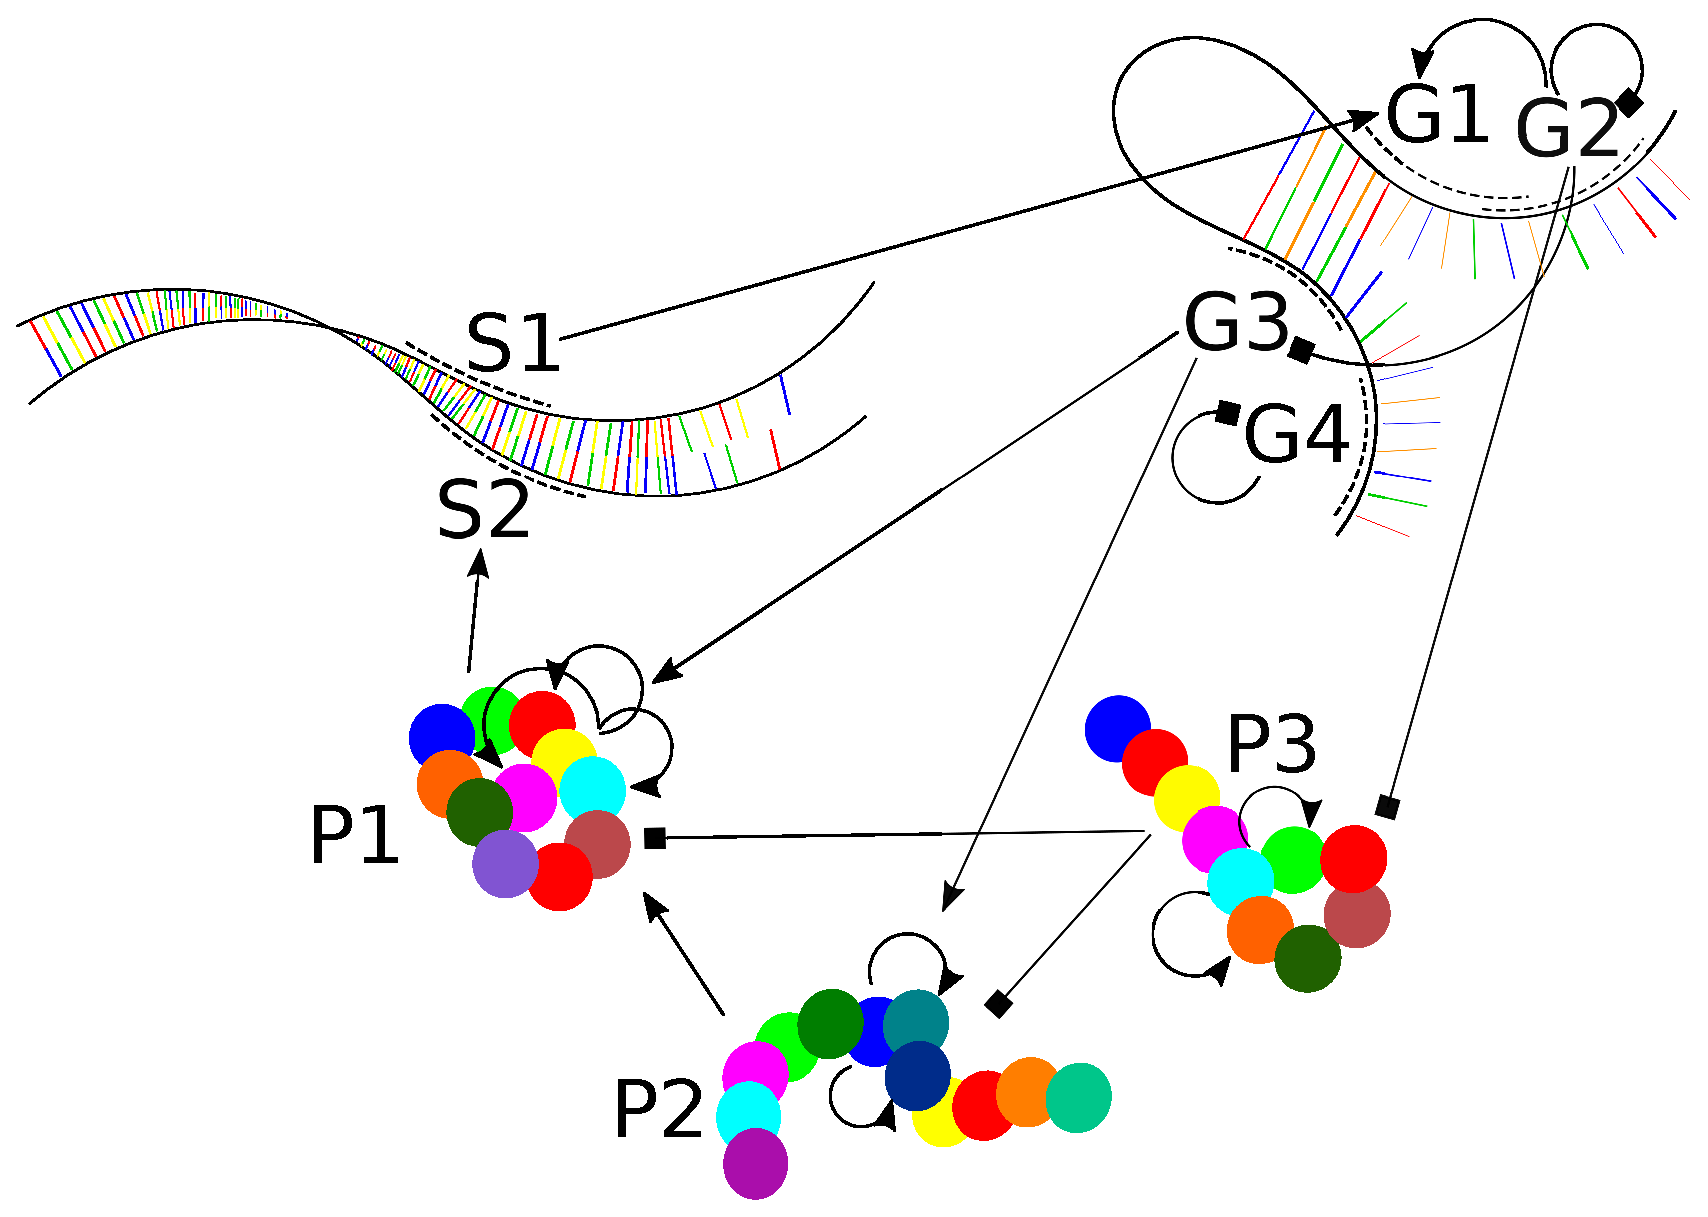
\includegraphics[width=1\linewidth]{2/DNA2.eps}
\caption{{\textbf Agnostic Biological Regulation.} Elements are seen to regulate one another regardless of biological mode/level, leading to loops as well as cascades of regulatory signaling. The regulation need not be direct, as this example contains no two factors directly linked but rather factors are linked between both the three distinct biological levels of DNA Sequence (S), RNA Gene (G) and Protein (P) as well as within level, \ie G2->G1, P3->P2->P1. In this example, S1 upregulates G1, which itself is also upregulated by G2, which concomitantly down-regulates G3 and P3. P3 would normally directly bind both P1 and P2, however the partial absence of both now limit upregulating expression of S2 to initiate further regulation (not shown).
}
\label{fig:DNA}
\end{figure}


\subsection{Implication}
\label{sec:practical}
A better understanding of the interplay between constituent regulators throughout every level of biology is crucial toward the development of any form of personalized or precision medicine \citep{barabasi2011network}. A recent study linked a large portion of human genes, some 17,000 to over 15,000 diseases, disorders or abnormal phenotypes \citep{pinero2015disgenet}, making for nearly half a million unique gene-disease associations. Only by placing these components together can we glean practical insights towards actionable intervention in the general systemic decay leading to disease onset, development and progression. Genotyping of certain disease markers simplifies the search-space in individual patients, making it possible to give reasonable developmental predictions, many of which have actionable responses to prevent any (further) future damage to the patient, \eg BRCA1 \citep{lerman1996brca1}. Such relationships are continually uncovered, revealing more of nature's order, enabling, for example, ever wider fetal defect screening for expectant mothers, such as heart defects \citep{hyett1999using} as well as for those in especially compromising climates around the world vulnerable to certain debilitating disease.

In addition to identifying biomarkers, such GRN can draw upon knowledge describing disease in other contexts, \eg correlating certain SNPs to complex traits \cite{platig2016bipartite}. While SNPs have classically been a resource bloating databases but seldom used to describe systems, in this way databases become enriched with new regulatory knowledge, opening SNP and other such isolated data to use by the community. Furthermore, new applications could developed, \eg more simply profiling new patients, expanding the use of this existing resource. 

Drug development is another area of personal interest and huge potential upon accurately mapping the interaction among biomolecules. Understanding the relationships present in a individual and tracking them as they change during disease development allows for one to uncover exact targets for drug intervention. It is not so simple to say once a target is known a treatment can be found, but it is has long been a necessary precursor of such development. What is more promising still is the targeting of gene modules, complexes or regulatory subnetworks so interdependent that knocking out one element alters the activity of the rest. Such targeting would offer a nevertheless real means of affecting change in patients without the extreme specificity required of singular targets. A growing field and a personal ambition lies in the use of, among other approaches, directed acyclic graphs (DAGs), \ie GRN, to screen profiles of compounds, to repurpose adverse side effects to affect change in disparate classes of patients. The more completely this interactive landscape is detailed, the more directly compounds targeting similar combinations of sites in antagonism with disease progression can be identified, not to mention the prospect of designing generic molecules. This lessened specificity would, however, bring concern for effects beyond design. Whether by repurposing, or repositioning, drugs tested to be safe for human consumption, or designing new drugs to treat new disease, accurate knowledge of the mechanisms underlying developmental paths toward disease are key, an aspect of which can be gleaned from reliable GRN inference.
				
% \externaldocument{4/chapter4.tex}
\section{Systems Dynamics}
\label{sec:sysdyn}
The modern understanding of biology has grown concomitantly with the means and methods by which to characterize every deeper and with more resolution the various biological levels of organization, \ie tissues, cells, organelles, protein structures, \etc. This is made possible, in part by developments in biophysics and biochemistry which usher in ever more fine grained probing technologies \cref{sec:bioreg}. % Inter- or intra- relationships between subgroup members can utilize analytical techniques from other disciplines and need not be reinvented. 
Similarly, the interdisciplinary field of systems biology has borrowed many tools from the domains of mathematics and physics. For example, the study of complex systems lends to analysis of \textbf{emergent} organizational structure leading to function which cannot be explained by investigating individual constituent components alone. In biology, a systems approach is needed to track the many collective, macroscopic effects individual interacting components spontaneously birth. Derived from the latin \emph{plexus} meaning intertwined, the ying to complexity\'s yang is separability. Reducing complex systems to components removes novel information regarding interaction and thus limits predictive capabilities on that same system. This is a major motivation for inferring the network at once using ordinary differential equations (ODE) rather than many mutual information (MI) methods which infer links individually in relation to one another, discussed in \cref{sec:models} on page~\pageref{sec:models}. Furthermore, our group has found several data properties to be strong indicators of the ability to correctly, accurately and reproducibly infer networks. The following offers a brief introduction to these relevant attributes as we have defined them, including sparsity, the signal-to-noise ratio, and condition number or Interampatteness discussed in \cref{sec:biosys} on page~\pageref{sec:biosys}.


\subsection{Two General Aims}
\label{sec:purpose}
In the landmark paper of its kind, Gardner and Faith \cite{gardner2005reverse},\cite{HECKER200986} offer descriptions of types of networks based on two aims. The first offers a \textbf{physical} view of direct binding interactions among biomolecules via chemical or other linkages. To leave a single biomolecule unquantified risks its activity being interpreted as that of another molecule, and thus this method is both highly expansive scope as well as rather dubious to characterize. Thus, a second \textbf{influential} approach is proposed, whereby indirect interactions are allowed by the added caveat that any measured interaction is necessarily not-direct. This type of network contains interactions capable of passing through innumerable intermediate biomolecules and indeed levels of biology on its way to affecting its eventual target. A major assumption of this research lies in the nature of the response to perturbation, \ie that the system has reached some state whereupon interaction between genes is stable and major change is less likely \cite{gardner2003inferring, faith2007large}. This surely simplifies reality but is quite powerful for modeling the large, overriding tendencies driving operations crucial to cellular life, and as such has seen extensive adoption in the field of systems biology.  These works form the foundation of the work and many of the ideas presented here. 
%build to the main points of \cref{sec:practical}
% \subsection{Time-Series}
% \label{time}
% % Time-Series

% Non-linear time series/ Michaelis-Menten/ hill kinetics Time
% LDS/ Linear

\subsection{Regulation is as much about \emph{what} as it is \emph{when}}
\label{sec:regwhatwhen}
Dynamics is in its most basic form a study of what and when -- by how much has any given system element changed over any given element of time. Determining these rates of change is the primary concern of experimental biologist wishing to better understand their investigative niche, for example. Together these niche experts can bind their individual biomolecules of interest together into a system using equations defining their rates of change in relation to one another using a \textbf{system of equations}. As with all models, there is a trade-off between the accuracy of your model and the complexity. The simpler the equations, \ie the fewer parameters and lower the complexity, the fewer degrees of freedom and by extension the fewer data points are needed to recreate the observed behavior compared to the more complex alternative. However, description of the given system can vary in appreciable ways depending on the modeling paradigm adapted. 
\textbf{Nonlinearity} presents the potential for higher resolution, but risks misrepresenting underlying biology by overfitting to input data. Systems by definition are closed, and as such, stability is born in the balance of growth and death, where degradation prevents system-wide collapse due to runaway growth\cite{alon2007design}. This can be carried out through feedback or feed forward `ms (see \cref{sec:pat}), alerting the system to the dangers of blindly continuing its present course without adaptation. Nonlinear models might be especially useful for modeling the robust capabilities of many natural systems to host multiple stable, \emph{steady states}, where overall change is null, \eg modeling diauxic growth of \coli on glucose and lactose \cite{wong1997mathematical} where the model must encompass for similar growth function under the presence of separate metabolite, see \cref{sec:stab}. 
Work has also been done to show that nonlinear systems, in which there is no proportional relationship between a given input and its effect on the systems output, can be approximated fairly well using the simpler linear models when the system finds a single steady state \citep{wildenhain2006reconstructing, crampin2006system}.  \textbf{Linear} relationships enable simplification at the cost of reflecting abstractions of truth. Simplifying the exemplified model to linearity might mean diminishing focus on individual metabolite levels and simply accounting for survival, \eg noting any lag period indicative of the bacterium trying to adjust to any limited resource before initiating death phase.


\subsection{Parameter Estimation}
\label{sec:parest}
A prerequisite to modeling any system is a means of mapping two sets of variables to one another. Convention dictates this function use various assemblies of parameters to equate independent and dependent variables. Thus we implement a linear model to determine the parameter values which will fit observed data to model outputs. Here our investigation is focused on changes in gene expression over time, and thus an element of time must be incorporated, making our models dynamic via implementation as \textbf{first-order} linear differential equations, \ie relying on the function\'s first derivative. Also, because the quantity we strive to characterize is non-static, \ie deviates over time, compounded by the fact that the measurements we gather are prone to error, elements of noise persist into our data, and so an estimation of noise is calculated for, as follows:

\begin{equation}
\label{eq:Linearmap}
  Y = -A^{-1}(P+F)+ E,
\end{equation}
% \myequations{Linear Map}

where the independent measurements Y map to the known experimental design P to solve for a GRN structure, A, which explains both while also accounting for systematic and model error, E \& F. As such, the rate of change defining the system's assumed steady state (after perturbation) is calculated as the sum effect of all other regulators for the gene. The model parameters we are solving for facilitate the mapping of variables to one another as defined by our input measurements, \ie an inverse problem, which we resort to solving using modern methods. Many methods can solve this problem, but an optimal minimum-variance, unbiased estimator (MVUE) for sufficiently large datasets remains largely elusive \citep{kay1993fundamentals}. As such, presented next are several methods which compete for the title of least bias and most accuracy. As one may guess, there are trade-offs between them which require the survival of the others, \ie no universal winner.



\subsection{Regression}
\label{sec:regress}
Gauss first devised the least squares estimation to study planetary motion in the late 18th century. Simply put, one uses regression analysis to see how a dependent variable changes with respect to an independent variable. Linear models such as \textbf{least squares} suffice in predicting relationships between input and output variables reasonably well, especially in cases of small sample size, low SNR or sparse data \cite[p.43]{friedman2001elements}. Such makes this \emph{elementary} approach particularly well suited here in this biological context. This carries known limitations, namely returning estimates with large variance and large state space, \ie accounting for variables which are not necessary to describe the ''big picture''\cite[p.57]{friedman2001elements}. However, least squares (LS) and our implementation have been improved upon using \emph{pseudo-inverse} functionality \cite{carlson1974generalization} to enable operating at such sparsities as GRN require. Additionally, this has been fit with an added constraint, a cutoff (LSCO) \cref{eq:LSCO}, where sparsity is given to the solution \emph{post hoc} in a stepwise manner determined by link confidence.

When fitting the data to the perturbation matrix with an estimated error on each, we seek to minimize the difference, the distance between the matrices, as in our linear model presented in \cref{sec:ODE}. Here we find Gauss' ideas and methods it has inspired similarly valid \textbf{regression} approaches (\cref{eq:LSCO} and a total LSCO (TLSCO) variant \cref{eq:TLSCO} \cite{de1998introduction} which carries out this minimization along both independent and dependent variables)%, detailed figuratively in \cref{fig:modelFit}) 
to minimize the residuals between the experimental measurements and the line when estimating parameters in our model (\cref{eq:Linearmap}). %Note that a perfect fit is largely held for theoretical realm, while overdetermined cases allow room for measurement error, etc.

%  \begin{subequations}
  \begin{equation}
       \hat{A}_{LS}={{Y^TY}^{-1} Y^TP}
 \label{eq:LSCO}
 \end{equation}
%  \myequations{LSCO}
%  \begin{equation}
%   \hat{a}_{ij} \triangleq \left\{
%     \begin{array}{ll}  a_{ij}^{ols} & \textrm{if}\; a_{ij}^{ols} \geq \tilde{\zeta}\\
%       0 & \textrm{otherwise}
%     \end{array} \right. \; \textrm{with} \; \mA_{ols} = -\bP\bY^{\dagger}.
%     \label{eqn:linLSCO}
% \end{equation}
% \end{subequations}
% \myequations{linearized LSCO}
\begin{equation}
  \begin{aligned}
%     \svd
    \lbrack Y P\rbrack &= U S V , \\
    \hat{A}_{TLS} &= -\frac{VYP}{VPP}
 \label{eq:TLSCO}
  \end{aligned}
 \end{equation}
% \myequations{TLSCO}
% \begin{equation}
%   \begin{aligned}
%     \gamma(a_{ij}) \triangleq & ~\sigma_{\breve{N}}\left(\mPsi(\chi)\right), \\
% %     \text{with each element}\nonumber\\
%     \psi_{kl}(\chi) \triangleq & ~\frac{\psi_{kl}}{\sqrt{\chi^{-2}(\alpha,\breve{N}\breve{M}) \lambda_{kl}}}, \\
%     \mPsi \triangleq & ~[\bphi_{1},\ldots,\bphi_{j-1},\bphi_{j+1},\ldots,\bphi_{\breve{N}}, \bxi_i]
%     \label{eq:RNI}
%   \end{aligned}
% \end{equation}
%  \myequations{RNI}

Recently, issues of scaling have since arisen as we have pushed to include more genes into our GRN. Specifically, we have hypothesize the lack of regularization in our LSCO implementation, which has led to our reliance on LASSO, described in \cref{sec:reg}, begets mega-hub regulator genes unrealistic in biologic systems \cref{fig:hubiness}. While there is undeniable bias in both methods, the extent to which LASSO creates unwarranted hubs of degree 30 is 10 fold less than that of LSCO at degree 250+. This is an ongoing and quite interesting problem to have stumbled upon, and results are unpublished. While the results are quite conclusive and broad-spanning (both in cases of synthetic and real datasets), no solution has yet been implemented.
% \begin{figure}[H]
% \centering
% 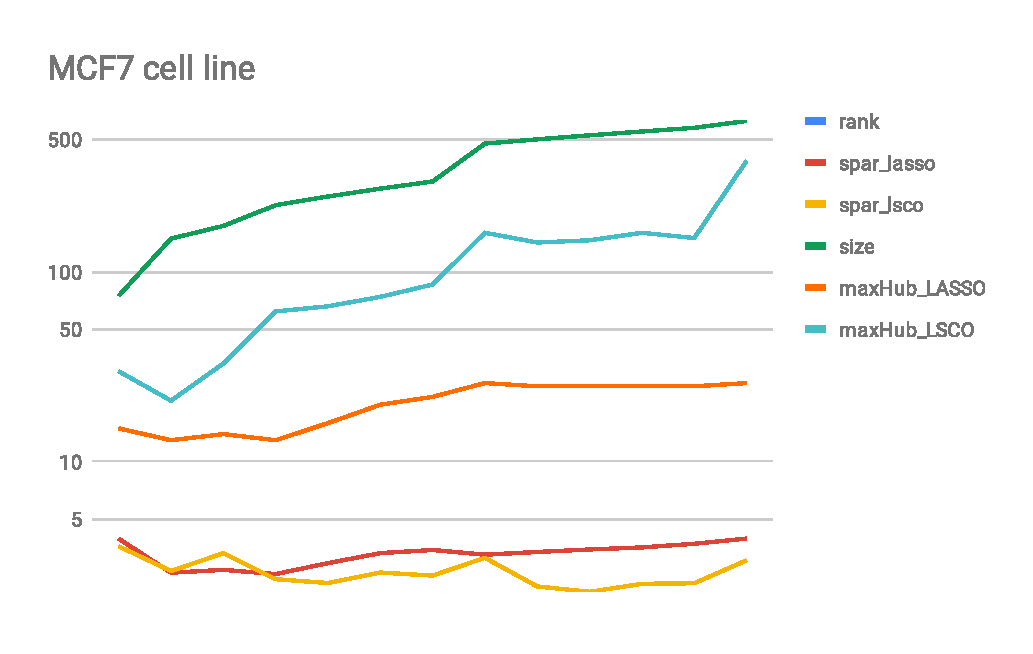
\includegraphics[width=.75\linewidth]{3/MCF7_cell_line.eps}
% \caption{\textbf{Summary comparing the maximum regulatory hub size as the MCF7 gene list is reduced.} Networks were cataloged when the average sparsity ranged between two to four links per node by both methods of inference. Note that rank and size being equal present overlapping lines, and thus only green is plotted. MCF7 is used as an illustrative example, however, this trend is present in all 11 tested L1000 cell lines as well as synthetic datasets.
% }
% \label{fig:scaling}
% \end{figure}

\begin{figure}[H]
\centering
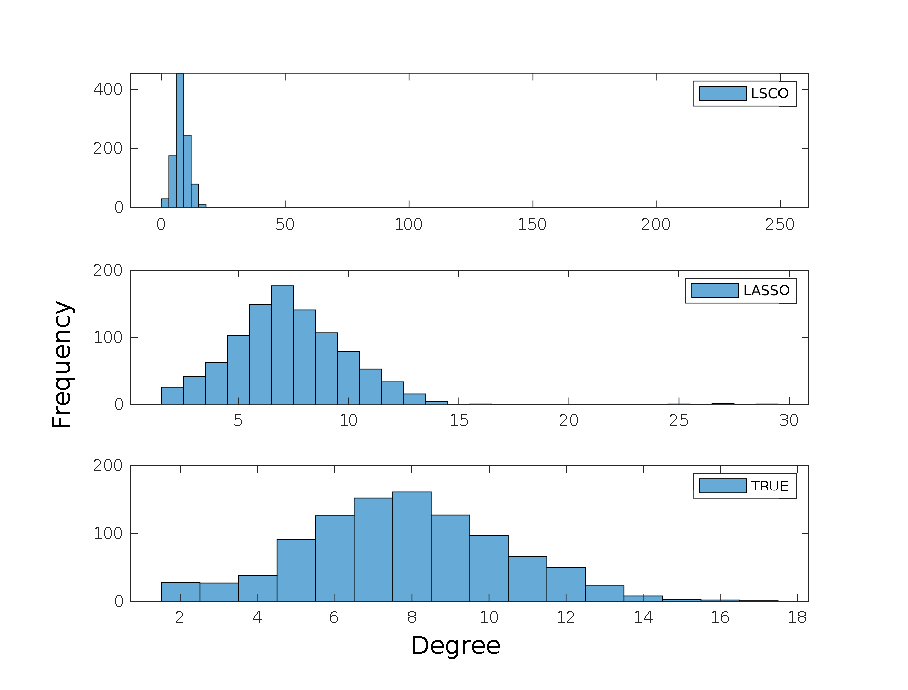
\includegraphics[width=1\linewidth]{3/hubs.eps}
\caption{\textbf{GRN node degree distributions per method.} A synthetic 1000 gene (N) network was created, where the true sparsity is $\alpha$=3.89, data synthesized and GRN inferred using both LSCO and LASSO, with sparsities chosen to match this truth as close as possible, at $\alpha$=3.978 and $\alpha$=3.676, respectively.}
\label{fig:hubiness}
\end{figure}




% Linear ODE- Least squares with penalty
% LASSO/ridge (L1,L2), Elastic net
\subsection{Regularization, OR penalized Regression}
\label{sec:reg}
Similar in aim but more capable when confronted with collinearity or seeking sparse solutions, several competing \emph{regularization} approaches exist, each with strengths, which under the right circumstances may outweigh any limitations \cite[p.69-73,661-668]{friedman2001elements}. LASSO (short for (least absolute shrinkage and selection operator) (\cref{eq:linLASSO},\cite{tibshirani1996regression}), Ridge Regression (also known as Tikhonov regularization, \cref{eq:ridge} \cite{hoerl1970ridge}) and Elastic-Net (El-Net) (\cref{eq:EL}\cite{zou2005regularization}) are, in effect, similar but distinct ways of minimizing this distance between matrices when regressing, summarized in \cref{table:regularization}. While elastic-net seeks to exploit strengths of both to overcome their individual weaknesses, lasso somewhat erratically picks one variable over the other, while ridge shrinks them towards one another for a more consistent, reproducible result \cite{ng2004feature}.

%  \begin{subequations}
%  \begin{equation}
%  \min_{w \in \mathbb{R}p}
%  \frac{1}{2m} \norm{\mA_i\mY^T+\mP^T_i}^2_F + \zeta \norm{\mA}_1
%  \label{eq:LASSO}
%  \end{equation}
%  \myequations{LASSO}
 \begin{equation}\label{eq:linLASSO}
 %\argmin_{\mA} \frac{1}{2m} \norm{\mA_i\mY^T+\mP^T_i}^2_F + \zeta \norm{\mA}_1 %\citep{Glmnet-LASSO}
  \hat{A}_{\textrm{LASSO}}(\tilde{\zeta}) = \arg \min_{A} ||A Y+P||^2_{L_2} + \tilde{\zeta} ||A||_{L_1},
\end{equation}

 \begin{equation}\label{eq:ridge}
  \hat{A}_{\textrm{Ridge}}(\tilde{\zeta}) = \arg \min_{A} ||A Y+P||^2_{L_2} + \tilde{\zeta} ||A||^2_{L_2},
\end{equation}

 \begin{equation}\label{eq:EL}
  \hat{A}_{\textrm{El-Net}}(\tilde{\zeta}) = \arg \min_{A} ||A Y+P||^2_{L_2} + \tilde{\zeta} ||A||_{L_1}+ \tilde{\zeta} ||A||^2_{L_2},
\end{equation}

Whereas least squares \cref{eq:LSCO} returns an estimate of fit for all variables which results in models which suffer from poor generalizability or issues of over fitting, regularization methods use a penalization in the form of a \textbf{cost function} to solve \emph{ill-posed} \cref{sec:calc} problems such as our inverse problem of inferring GRN from expression and design matrices. Choosing the right model returned by LASSO or Elastic-Net then becomes a game of comparing predictions to some ground truth, usually left-out training data, \ie via cross validation referenced in \cref{sec:calc},\cref{sec:acc}.

\begin{table}[H]
\begin{tabular}{|l|l|l|l}
\cline{1-3}
 & \textbf{Lasso} &  \textbf{Ridge} &  \\ \cline{1-3}
\textit{norm} & L1 &  L2 &  \\ \cline{1-3}
\textit{selection} & sparse  & shrinks &  \\ \cline{1-3}
\textit{scaling} & not independent &  independent &  \\ \cline{1-3}
\textit{constraint} &sum of absolute coefficients& sum of squared differences&  \\ \cline{1-3}
\textit{penalization} & more uniform &  larger preferred &  \\ \cline{1-3}
thresholding & soft &  hard &  \\ \cline{1-3}
\end{tabular}
\caption{Comparison among L1 and L2 regularization techniques}
\label{table:regularization}
\end{table}

\subsection{Calculability}
\label{sec:calc}
Several methods exist for solving minimizations problems, not limited to those lsited in \crefrange{eq:LSCO}{eq:EL}, however unique parameter estimations are not guaranteed. Such cases are denoted \textbf{underdetermined} and deemed \textbf{nonidentifiable}; here the specific case of inverse problem solving returning non-unique solutions requires additional assumptions, \ie are \textbf{ill-posed} problem. Both biological and technical replicates can help to decrease uncertainty in such estimates \citep{lee2000importance}. Furthermore, biological replicates enhance the utility of \textbf{bootstrapping} by expanding the creative potential for new datasets to estimate parameters. Assuming any systemic noise is both uniform and independent, such repeated experiments offer estimations of both true variability of the biological system as well as of noise implicit to the characterization system. Disambiguating these quantities is not trivial. Thus, expanding the number of measurements in the form of \textbf{resampled} datasets is one way to improve the parameter estimation, returning a better estimate of the parameter space. However, the model loses its ability to generalize,\ie to reliably predict new data, when more data is used for parameter estimation as the risk of overtuning arises. For this reason, a simple solution can be made by removing portions of individual datasets, training on only a random portion, which you shuffle around across many calculations. Such \textbf{cross validation} techniques are widely used in modern \textbf{machine learning} practices. A caveat to such practice, however, is that by requiring more calculation... you require more calculation, and thus more time. Depending on the underlying estimation efficiency (LSCO \cref{eq:LSCO} compared to something like LASSO \cref{eq:linLASSO}), this can amount to quite large increase overall compute time.


% \begin{figure}[H]
% \centering
% 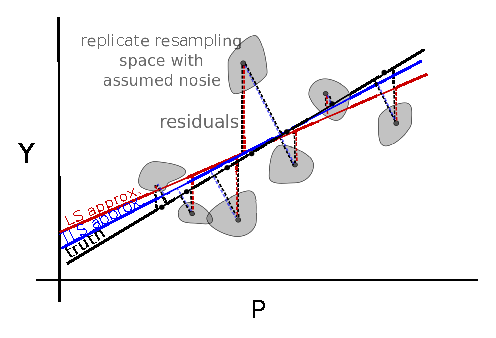
\includegraphics[width=.75\linewidth]{3/model_fit.eps}
% \caption{{\textbf Comparing residuals from regression methods.} Red lines show least squares and blue lines total least squares accounting for both independent and dependent variables. Grey areas around points illustrate zones of uncertainty probed by bootstrapping experimental replicate points.
% }
% \label{fig:modelFit}
% \end{figure}

\subsection{Network Inference}
\label{sec:netinf}
Networks arrange information regarding the interactions of constituent members in a manner prone to statistical analysis and often aid in human understanding. In the context here, a node is generally in reference to a singular biomolecule, be it transcription factor, gene, intermediate gene product, protein, \etc, which plays some role in the regulation of another such factor. Regulation comes about by a binding interaction of some sort dictated by the level of biology. This relational information is conveyed as a weight, the degree to which one factor influences another, and can either convey up- or down- regulation.

Several approaches exist for this reverse engineering, ranging from an outdated assembly of one-to-one relationships to correlating patterns throughout expression assays,\etc. Some inference methods return link existence with no confidence or weight, so called \emph{binary networks} (see \cref{sec:models}). In this and other scenarios, link weights can be estimated after link existence is establish. Such was the case after the creation of a null inferred network distribution, as in \textbf{Paper II}. In that study, however, struggling to find a representative null distribution realistic enough to compare to and thus implement an FDR restriction, we refit inferred, shuffled network links using constrained least squares (CLS, \cref{eq:CLS}, \cite{grant2008cvx} in the context of \cref{eq:Linearmap}) to improved their performance against measured links (detailed in the authors note in \cref{note}). 


\begin{equation}%\label{eqn:CLS}
\begin{aligned}\label{eq:CLS}
  \hat{A} = \arg in_{A} & \sum \diag(\Delta^TR \Delta), \\
  \text{s.t.}\; & \Delta = A Y + P, \\
% \label{eqn:CLSPredErr} \\
  & R = \left( \hat{A}_{\textrm{init}} \Cov[y] \hat{A}_{\textrm{init}}^{T} + \Cov[p]\right)^{-1},\\ %\label{eqn:CLSR} \\
  & \sign{A} = \sign{\hat{A}_{\textrm{reg}}}. \\
%   \label{eqn:CLSStructure}
\end{aligned}
\end{equation}
% \myequations{CLS}

This process is contained within the general balance fit error (BFE) algorithm in \textbf{Paper III}, wherein this optimization is iterated for balancing among input and output errors. This is done in order to minimize the overall error of the network reproducing the dataset in a leave-out manner, while still accounting for error inherent to the creation of the perturbation design matrix used in our linear model (\cref{eq:Linearmap}).

\subsection{Comparison to Null: Limiting Random Artifacts}
\label{sec:null}
The novelty and power of both \textbf{Paper II} and \textbf{Paper III} is drawn from a comparison to a null distribution of shuffled data and shuffled links, respectively. Networks inferred from shuffled data offer an estimate of how likely it is by chance to retrieve any given link by random chance. Constructing a consensus network in comparison to these random-chance links as we did thus restricts them links from inclusion. These links likely constitute false links, and as such inclusion in the final network would do so at the cost of increasing the \textbf{false discovery rate} (FDR) \citep{kall2007posterior}. In a similar way, testing how well shuffled GRN reproduce independent datasets allows testing of significance of how well a GRN inferred from real data can do the same. These null distributions are admittedly na{\"i}ve, but nevertheless have been shown to provide real improvement through their implementation in various pipelines here and elsewhere. Specifically, note such a null distribution is constructed from $10^5$ permuted label versions \cite{platig2016bipartite} in the COPD case study within the CONDOR publication for a similar comparison, lending significance to GWAS SNP data used to infer regulatory relationships between and among genes (see \cref{sec:practical}).	
% \externaldocument{2/chapter2.tex}
% \externaldocument{3/chapter3.tex}
\section{Biological Systems}
\label{sec:biosys}
The process of science is at its core nothing but a method to isolate phenomena to singular factors to attribute a cause to an effect. However, as we have seen, such isolation can be detrimental to the accuracy of the observation being gleaned. Thus, many if not all fields of science have long applied analytic tools developed alongside various branches of mathematics to ensure that while many factors are considered, their main observation is the most likely result of some initial cause. So too systems biology attempts to further quantize the realm of biology to more reflectively model natural systems in their native state, accounting for ever more variables in the process while maintaining confidence in the correlation of their experimental outcome.

\subsection{Stability}
\label{sec:stab}
As alluded to in \cref{sec:regwhatwhen}, natural systems have the ability to fluctuate in response to any number of internal and external stimuli, \eg up-regulating heat shock protein (HSP) in response to excess heat. In a similar manner to new growth media spurring rapid growth in bacterial cultures only to plateau and eventually die off if left alone, this HSP up-regulation is a momentary disturbance from a previous balance, a state of intermediate HSP levels, stable enough to call for more or less as the situation should demand. In characterizing HSP level in response to excess heat, one might expect a large increase in mRNA levels while heat persists. Similarly, after targeted gene knockdown, mRNA levels of said gene gradually decrease as indirect gene partners feel the effects of their partners decreased presence. A state of zero net change is only reached after the system has adapted to this new, decreased but not characteristically altered state as time is allowed to run (\cref{fig:SS}).

\begin{figure}[H]
\centering
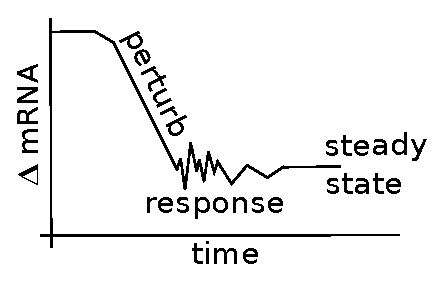
\includegraphics[width=.5\linewidth]{4/pert.eps}
\caption{\textbf{Arrival at steady state after perturbation.} Over time a system will recover from the shock of its initial perturbation to reach some altered, new steady state.
}
\label{fig:SS}
\end{figure}

The assumption of biological systems stability is best framed in view of the alternative hypothesis, that is if systems were unstable, any minor variation, over time, would lead to system collapse \citep{khalil1996adaptive}. A simple way to ensure stability in any dynamic system, and in fact quite a divisive topic in the inference community in particular, is the inclusion of self-regulation in the network. The self interaction plays out indirectly as regulators are transiently expressed to carry out some function, they must then be degraded to reduce cease this response functioning. For example, self-regulation through degradation may be achieved as a secondary effect, wherein buildup of a sought after heat shock response element reaches a critical threshold wherein a cleavage factor creates a byproduct which then binds to the upstream promoter region to shut down heat shock response it partially helped initiate. The cyclic nature of regulatory pathways (\citep{yi2000robust}, see \cref{fig:DNA}), relationship can be seen as inversely proportional, for the quicker this initial factor is expressed, the more of it will surpass this threshold before actively stopping its production and cleavage. Depending on the time delay before byproduct expression and activity is felt, more or less byproduct will be available for cleavage to signal slower or faster overall heat shock response death. This simple indirect feedback mechanism, in concert with other factors, can control quite complex cellular features, such as are described in \cref{sec:pat}. A handful of inference methods disregard this auto-regulatory behavior altogether (ARACNe \citep{montes2014aracne}, CLR\citep{faith2007large}, Genie3\citep{GENIE3}, PLSNet\citep{ham1996partial}). Still others insist on a large portion of measured genes carrying out self-regulation to some degree, ensuring their own expression does not go unchecked, thus destabilizing the system.

As detailed in \textbf{Paper II}, several (penalized) regression based GRN inference methodologies implicitly consider the stability of the system they infer. \textit{Stability selection} uses LASSO under randomized parameterization \citep{tibshirani1996regression} in combination with the irrepresentable condition \citep{zhao2006model,jia2012preconditioning}. More reliable GRN inference was demonstrated under a stability criterion by choosing links with subsampled frequencies above an expected upper false positive boundary,  \citep{meinshausen2010stability}.  \textit{Random LASSO} \citep{wang2011random} improves link selection by averaging across bootstrapped distributions of randomly selected subsets of the data, while \textit{TIGRESS} combines stability selection with iterative least angle regression (LARS) estimation \citep{haury2012tigress}.

\subsection{Patterns}
\label{sec:pat}
Life may be presented with any number of stimuli at any given time, and it is only through the mechanism of evolutionary discovery that an adequate response is reached. The cell has many tools to combat an external offense, triggering unique patterns of interaction amongst numerous individual components as an innate response mechanism occurring on a scale of time deemed necessary by evolutionary predictability, \ie what has allowed for survival before. These individual component \emph{motifs} and their respective responsiveness flow into and out of one another to compose increasingly complex mechanisms of survival. Examples of motifs studied in \coli  and \yeast alike are \emph{feed-forward loops} (FFL) and \emph{feedback loops} (FBL).  FFL can amplify the response to an initial stimuli resulting in a quicker response to a potentially deadly threat, while FBL can help to stabilize such response after time has been allowed for its effect to carry out by targeting the very factor initially called for in response to the stimuli to be regulated in the opposite direction initially called for in response \citep{milo2002network,mangan2003structure}. Others motifs include multi- and single- input module (MIM/SIM), dense overlapping regulons (DOR), and regulator chains \citep{kalir2005coherent,lee2002transcriptional,wang2010process}. Other methods of robust adaptation in  \coli include bistable systems featuring hysteric behavior where feedback coefficients are greater than one, and oscillatory behavior regulating systems at levels of complexity as high as circadian rhythms \citep{szallasi2006system}.

Motif patterns are identified by comparison to random and are thus agnostic of node makeup, and thus should not be confused with a network module. \emph{Modules} are composed of select genes \eg to perform distinct functions including transcription and signaling, and are thus seen to be highly conserved across species \citep{alon2007network}. Completely connected subgraphs, known as cliques, appear as motif elements in \yeast at a conservation rate of nearly 50\% among five higher eukaryotes, often sharing a common functional class \citep{wuchty2003evolutionary}. This would indicate that some patterns, specifcally those involving all elements in some way regulating all other elements, are so advantageous that in certain circumstances gene function is preserved through huge extents of evolutionary time.

\subsection{Properties}
\label{sec:prop}
\subsubsection{Condition}
\label{sec:cond}
It is important to distinguish data properties from systems (network) properties. Systems generally account for their ability to handle noise by estimating the worst case scenario for noise to change the system structure. The distinction is made in network inference of terming this conditioning as \emph{interampatteness} (IAA, short for INTERactions enabling simultaneous AMPlification and ATTEnuation of different signals), to call attention to it in more general dynamic systems and nonlinear environments \citep{nordling2009interampatteness}. Furthermore, the former is an inherent biological network property while the later also depends on the experimental design matrix.  Thus this interampatteness degree is a measure of the ability of the system to amplify certain signals while attenuating others whose signal is often riddled with systemic noise. This property feeds nicely into another, related property (see \cref{sec:rank}) which is also concerned with multicollinearity, wherein features are functions of one another.

\subsubsection{Rank}
\label{sec:rank}
Rank is another property worth consideration in the context of network inference, specifically in the subcontext of the generation of synthetic data and bootstrapped datasets. As aforementioned, we seek to infer networks where all genes regulate or are regulated, \ie a system in which each constituent plays a part. Therefore, if any two or more genes share highly correlated patterns among their readout genes when perturbed, their component system is seen as containing redundant information, \ie the system is \emph{rank deficient}. It is therefore, firstly advantageous to design datasets composed of genes likely to act and respond independently from one another, as the information content of the dataset is then maximized among the measured genes \citep{subramanian2017next}. Here we further ensure full rank of either matrix type so to guarantee experimental independence and thus prevent inference using less informative datasets. It has been shown that measuring more variables than are experimented upon, and vice versa, is a recipe for lessening the information content of a dataset \citep{Nordling2013}. This simple but computationally non-insignificant, preventative step assures users not remove information from a system.  If the angle of any genes pair combination is too narrow (\cref{fig:dend}) reduction should be done to remove redundant information from the dataset lest it risk being ill-conditioned or rank deficient.

\begin{figure}[H]
\centering
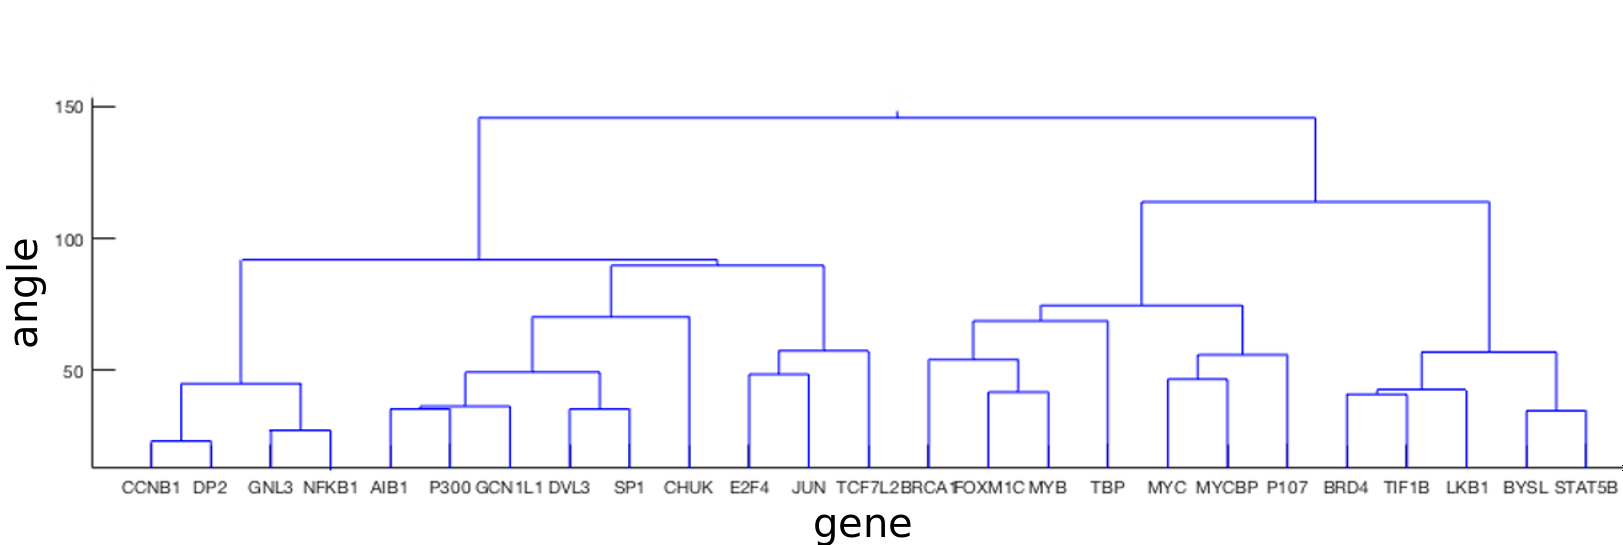
\includegraphics[width=1\linewidth]{4/MYC_Y_weightedDouble_dendrogram.png}
\caption{\textbf{Abbreviated view of MYC double perturbation angle dendrogram}. An example demonstrating independence of gene expression via correlation in dataset.}
\label{fig:dend}
\end{figure}

\pagebreak

\subsubsection{Noise}
\label{sec:snr}
As we have seen, systems are often riddled with noise, relying on mechanisms to maintain sufficient conditioning \cref{sec:cond} and rank \cref{sec:rank} to regulate survival; those investigated here are no exception. While noise has been confronted is some methods more directly\citep{zhang2012narromi}, we aim to \emph{handle} such noise, much the way the natural system does, and its effects on our modeling as it is partially a byproduct of the naturally robust biological system, made worse through the imperfect methods of quantizing a continuous, dynamical system at a single point, not to mention the quantification machinery. Simulating noise is thus equally crucial, and thus we implement a normally distributed model of noise, based on the standard deviation witnessed within measured expression to approximate this inherent noise. Recent findings suggest this may not be optimal, but it allows our models to dynamically represent possible sources of error when inferring networks, which flexibility would not be as forgiving in its absence.

Experimentally, we estimate the \emph{Signal-to-Noise Ratio} (SNR, \cref{eq:SNRl}). of the system assuming normally distributed noise as follows,

\begin{equation}
	\SNR_{\mY\, \normall} \triangleq \frac{\underline{\sigma}(\bY)}{\sqrt{\chi^{-2}(1-\alpha,NM)\lambda}},
  \label{eq:SNRl}
\end{equation}

where $\underline{\sigma}$ represents the smallest non-zero singular value, $\normall$ the normal distribution with mean $\mu$, variance $\lambda$ and $\chi^{-2}(1-\alpha,NM)$ is the inverse chi-square distribution with \emph{NM} ($genes \times experiments$) degrees of freedom at significance level $\gamma$ as defined in the supplement to \textbf{Paper I}.

In the case of simulation, wherein a network is initially created, datasets of various data property makeups are created by scaled SNR, a process that defines the E matrix. As such the SNR calculation is more straightforward and exact, where the smallest singular value of Y divided by the largest singular value of E (\cref{eq:SNRt},\cref{fig:SNR}).

\begin{equation}
    \SNR_{\mY\,true} \triangleq \frac{\underline{\sigma}(\bY)}{\overline{\sigma}(\bE)}.
  \label{eq:SNRt}
\end{equation} 

% \begin{wrapfigure}{Hr}{0.5\textwidth}
\begin{figure}[H]
  \begin{center}
    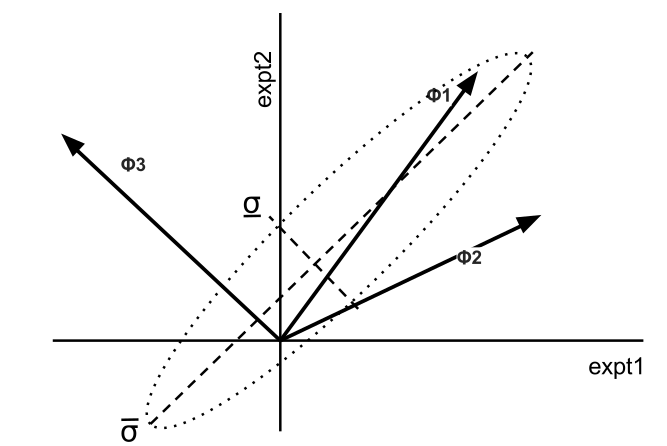
\includegraphics[width=1\linewidth]{4/matrixSNR.png}
%     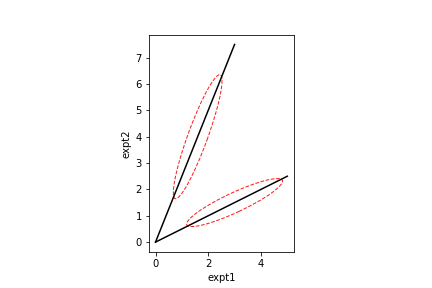
\includegraphics[width=.5\linewidth]{4/SNR.png}
  \end{center}
  \caption{\textbf{Regression lines of two experiments with ellipsoid SVD.} We make the conservative assumption that the minimum eigenvalue across the geneset is a fair proxy to calculate signal-to-noise (SNR) in relation to what is expected under the null $\chi^{-2}$ distribution.}
  \label{fig:SNR}
\end{figure}

\subsubsection{Sparsity}
\label{sec:spar}
The field of network inference aims above all else to determine interactions of consequence, those which affect other system constituents rather than laying idle and isolated. As such, the task must consider to which degree to consider a link is deemed valid, to what degree it initiates a response in its neighbor(s), \ie its link weight. This is done in many methods at once, by a sparsity parameter, $\zeta$, which incrementally returns networks of lesser or greater link weight, as determined by the inference method itself, creating a gradient of networks of increasing \emph{density} (decreasing sparsity) as weaker link weights are forced into inclusion (\cref{fig:confusion}). Finding the optimal sparsity is an ongoing field of research \citep{tjarnberg2013optimal}. Several different methods were employed throughout this work to determine a single, \emph{best} inferred network, often for comparison between methods or for heuristic reasons of biological relevance (\ie generally containing 3-4 links per node \citep{tjarnberg2013optimal}).The number of nonzero elements is limited using methods which place constraints on total link numbers, \eg the L1 norm in LASSO (\cref{eq:linLASSO}, discussed in depth in \cref{sec:reg}) and a cutoff for ordinary least squares LSCO and total least squares (\cref{eq:LSCO},\cref{eq:TLSCO}, and \cref{sec:regress}). Our R shiny web app ``CancerGRN'' (\cref{fig:GSweb}) which employs several network viewers to display networks at each sparsity level, a few crucial network properties, as well as displaying the overlap support plot for those GRN inferred using \emph{NestBoot} via \textbf{Paper II}.


\begin{figure}
\centering
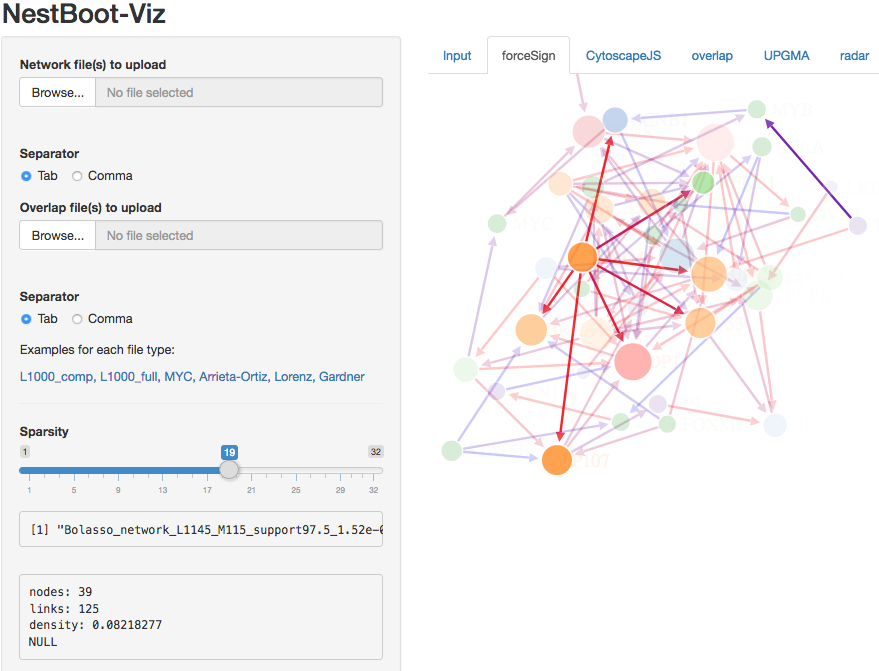
\includegraphics[,trim={0 0 0 1cm},clip,width=1\linewidth]{4/NestBoot-Viz2.png}
\caption{\textbf{Screenshot of Network Viewer CancerGRN Tool.} It offers a network view of variously sparse networks returned from inference, in addition to NestBoot support plots and several general network properties or statistics for comparison. \url{https://dcolin.shinyapps.io/cancerGRN/}, further capabilities demonstrated in \cref{fig:UPGMA}.}
\label{fig:GSweb}
\end{figure}

\subsection{GRN Modelling Architectures}
\label{sec:models}
As we have discussed, there are many approaches that can be taken to understand relationships among biomolecules. Generally inference methods can be categorized into four model architectures: boolean, bayesian, information theoretic and differential equations \citep{HECKER200986,xiong2012gene,yaghoobi2012review}. An overview of the latter three follows the cursory allusion to information theoretic methods in \cref{sec:sysdyn} and the introduction to ODE detailed in \cref{sec:parest}.

% \subsubsection{Probabilistic/Boolean/Petri Nets (PNs)}
% \label{sec:prob}
\subsubsection{Information Theoretic}
\label{sec:info}
The \emph{tree-based} method Genie3 \citep{irrthum2010inferring} uses the equivalent of \emph{supervised} (\emph{non-parametric}) learning feature selection to determine those genes directly influencing expression patterns of other genes, ranking such features via the tree building process. Thus, it is able to account for \emph{multifactorial}, \ie unknown perturbation, in the hope of finding genes with expression predictive of target gene expression. As we have seen, this is quite opposing the majority of investigated methods herein, regression methods requiring a perturbation design matrix. The \emph{ensemble} approach used in Genie3 improves prediction by averaging among bootstrapped trees, each a part of the initial sample space iteratively fragmented from logical demonstrations of single input variable.

\emph{Mutual information} based inference methods generally define a similarity metric between profile patterns of any two genes, a marginal dependency or \emph{coexpression}, on a gene-by-gene pair evaluation basis. An obvious distinction arises in that any such method differs from the {\it all-at-once} approach of regression methods \cref{sec:regress} such as LASSO, (Total) Least Squares, \etc. Relevance networks set a threshold above which any regulatory gene pair is identified as a link as a form of clustering \citep{faith2007large}. ARACNe implements an information-theoretic property, the data processing inequality (DPI), to threshold indirect links, seeking to increase true positive recovery while minimizing false positives. Below a certain DPI, the lowest link of three completely linked nodes is removed; otherwise the triangular clique is maintained \citep{montes2014aracne}. CLR, short for Context Likelihood of Relatedness, likewise utilized mutual information (MI) between all genes to estimate likelihoods for each compared to a MI background distribution. This null model is constructed from the MI sets between all possible links, most being that of random background MI due to biological GRN sparsity \citep{faith2007large}. In short, it applies normal distribution statistics to mutual information scores in order to identify network links. (B)C3NET \citep{altay2010inferring,de2012bagging} corrects for all possible inferred links via a maximization step where they ``bag'' significant links after hypothesis testing.

Several problems arise reading relational information in this way, least of which is ambiguity in the nature of the cause and effect. Imagine the unique GRN implied by one three node coexpression clique with no manner of discerning among the possible distinguishing features, \eg $A\to B\to C$ versus $ B\to A\to C$ \citep{markowetz2007inferring}.
Graphical Gaussian models (GGM) are examples of full conditional, undirected probabilistic network models estimated from a covariance (\ie concentration or precision) matrix, which \emph{partial correlation coefficients} are taken as directed, regulatory edges. This partial correlation acts as the strength of the direct, indirect or joint interactions between biomolecules. Whereas correlation networks return degrees of correlation for most genes, drowning out weaker dependent correlation by thresholding for high independent correlation, GGM return more likely interdependent regulations\citep{schafer2004empirical}. However, issues of rank and sparsity arrise when such GGM-based methods scale to larger datasets. In a logical progression toward independence of all orders, \emph{Bayesian networks} (BN) return directed links between given variables, and are thus distinguished as being DAGs representing interaction probabilities between multiple biomolecules. Partial DAGs are also used to collapse unique but equivalent skeletons of the same structure, \ie directionality is disregarded for all links showing bidirectionality between models.


\subsubsection{Perturbation-based Inference}
\label{sec:ODE}
A fundamental element of the inference contained within \textbf{Paper I-IV} lies in their experimental design, namely that response is measured after the system is given time to adequately respond to, \ie reach steady state, an external stimuli, namely a directed knock-down suppression of a gene expression \citep{pinna2010knockouts,oates2012network,yip2010improved}. The technique used to perform the knock-down (KD) is also not immune to introducing error. KD via short hairpin RNA (shRNA) and small interfering RNA (siRNA) are designed to target genes. However, given the robust flexibility demonstrated of biological systems to this point, it stands to reason that even primers targeting specific sequence, like the genes they preclude, are not entirely unique, and indeed are repurposed through the genome \citep{ye2012primer}. As such, several such primers which identify the target RNA sequence to suppress are either pooled together after reading or introduced as a cocktail, respectively, to mitigate off-target effects. In this way, all genes are systematically targeted with relative affinity, and the expression of readout genes (those not knocked down) are measured. This is a delicate yet imprecise balancing act, where one seeks mitigation of singular effect without irreparably altering the system, rewiring its connections and measuring an altogether different system. 

As is expertly stated in the 2018 Blum \etal publication, ``Inferability of a directed link between source and target node requires that the remaining network may not contain the same information that is transmitted between them. A sufficient condition is that all information that the remaining network receives from the source node is destroyed by sufficiently strong perturbations. If the target node is not perturbed, information from the source node may reach the remaining network through the target node'' \citep{blum2018experimental}. As such, the synthetic datasets contained with papers presented here \textbf{Papers I-IV} more strictly adhere to this absolute principle. However, real experimental knock downs only achieve this in part, and to varying degrees at that (see Fig. S2 in the \textbf{Paper III} supplement).

Furthermore, unlike correlation or mutual information based methods searching link-by-link to gradually forming a topology, inference using perturbation-based methods is an {\it all-at-once} procedure, \eg LSCO, TLSCO, LASSO (\crefrange{eq:LSCO}{eq:linLASSO}). Such methods here utilize a known experimental design in the form of a experimental design matrix, \ie $\mP$ to better inform the mapping of experimental dataset to the network structure. This design matrix links fold change patterns to interaction pairs in the network. Additionally, it aids in synthetic dataset creation, the network inference process run in reverse, a hugely important feature of the GeneSPIDER toolkit as well as the work contained here. Whereas Genie3 is designed to account for multifactorial unknown or undefined perturbations, here perturbations must be explicitly stated in this design matrix to be taken into account in the inference of an overall GRN topology. 
% Our linear methods are able to account for known perturbation designs orders greater than one as exemplified in part one of our validation study for the perturbation inference study (\cref{fig:meandouble}). 
The \emph{ensemble} learning based ENNET also relies on experimental design matrix, but to a different effect, considering it when TFs are estimated to target individual genes. Each such subproblem is solved using Gradient Boosting Machine which estimates TF importance or ability to regulate targets, which are evaluated systematically \citep{slawek2013ennet}.

\subsubsection{Integrative Methods and Bipartite Graphs}
\label{sec:bipart}

The value and meaningfulness of any given network increases as it more accurately reflects the true dynamic nature of any given biological system. Thus as more platforms are born it is not only advantageous but necessary to integrate this disparate information into a single network, be it GRN or other when considering \eg proteomic data, \etc. In this way, \emph{Fused regression} \citep{lam2016fused} weighs various levels of biological data with overlapping data points by their quality to integrate several data types to more accurately reverse engineer given regulatory networks. In this way, and in conjunction with the lab's \emph{Inferelator}\citep{bonneau2006inferelator} inference method, the fused regression package allows the integration of many biological levels of data toward inference of the network encompassing the amassed data, returning a more relevant and biologically meaningful network for its efforts. However, for its strengths, it is reliant upon an initial orthology for how to communicate relationships between and amongst the differing data level elements, ie mapping genes to their respective TFs in the form of expression values, block matrix of transcription factor expression values and regression coefficient values which define the regulatory relationships between TFs and their target genes. Their approach  calls for parameter optimization in addition to using L2 penalization followed by thresholding to return a similar sparsity gradient as L1, while also ranking interactions more accurately.

Similarly, PANDA (Passing Attributes between Networks for Data Assimilation) initiates a cooperativity network based on reliance of three levels of biological data -- TF, protein-protein interaction and sequence motif to represent responsibility via outgoing influential links and availability or the incoming ability to be regulated. In this way Glass \etal \citep{glass2013passing} are able to reconstruct genome-wide, condition-specific regulatory networks by weighing and integrating these data in a manner which cross-checks the \emph{availability} of a target gene to be regulated by a TF against its likely the \emph{responsibility} a TF is measured to have in regulating that gene. Somewhat of a limitation lies in the ability to weigh sources of data relative to their noise level, or any other criterion; however this is easily remedied before incorporation of various data into the final GRN.

\subsection{Methods for Network-Network Comparison}
\label{sec:net_com}
A link-by-link comparison between networks \cref{fig:dend} suffers from the same shortcomings that ultimately limit differential expression analysis (DEA), namely that each piecemeal approach isolates the most highly functioning links or genes, disregarding the state space within which these elements carry out their action. Each analysis is ultimately a study of driving forces defined by fundamental changes in the respective GRNs. Therefore any single gene-gene links on its own cannot suffice when seeking to understand systems dynamics, and instead links between highly differential elements must be preserved and compared, in the form of clique or module comparison. Whats more, these highly interacting and interdependent groups form larger targets as potential biomarkers for therapeutic intervention, wherein knocking out or perturbing in some way one element of a module could more feasibly bring about a positive response than the more strict targeting of single, unrelated gene lists returned from DEA or the link-by-link comparison.

% \begin{wrapfigure}{Hr}{0.75\textwidth}
\begin{figure}
\centering
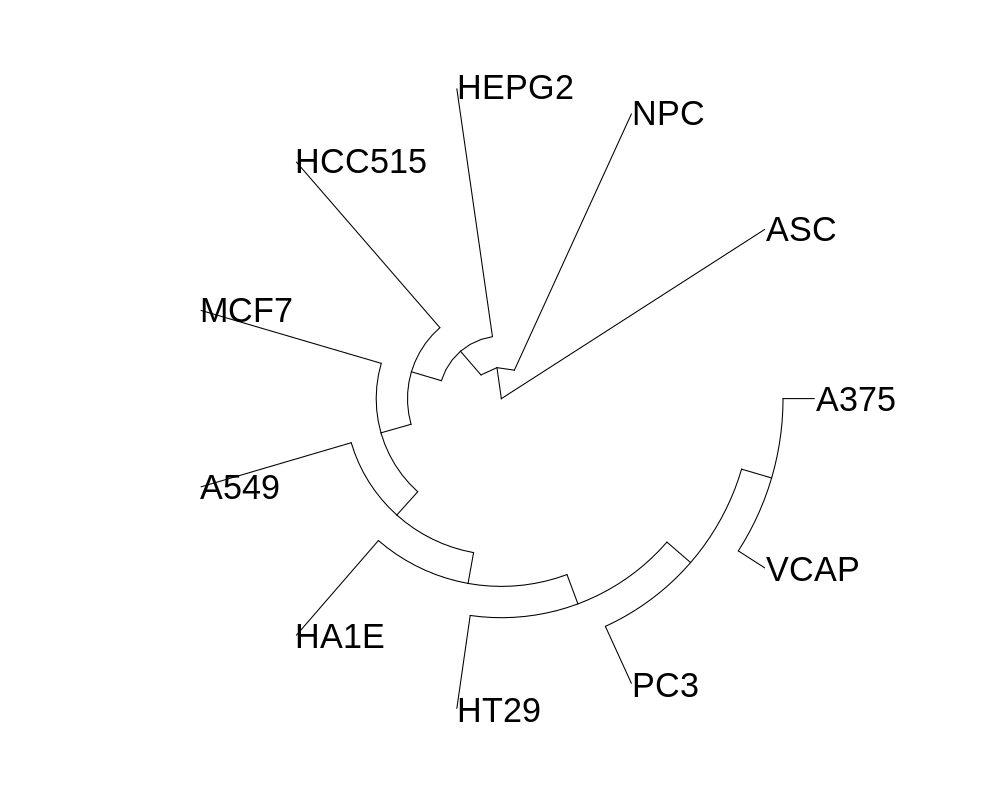
\includegraphics[width=.75\linewidth]{4/dend.png}
\caption{\textbf{Example of link-by-link GRN comparison as dendrogram.} Comparing initial LINCS cell line NestBoot GRN from early investigations of \textbf{Paper IV}, in an unrooted, circular configuration, as part of expanded UPGMA capability of the cancerGRN tool (\cref{fig:GSweb})}%. Live at \url{https://dcolin.shinyapps.io/cancerGRN/}}
\label{fig:UPGMA}%\end{wrapfigure}%{Hr}{0.5\textwidth}
\end{figure}

Beyond na{\"i}ve link-by-link comparison, there exist sundry methods for comparing modularity between networks of various levels of sparsity, \eg derived from different time points and obviously between healthy and disease derived cell line. CONDOR (COmplex Network Description Of Regulators) \citep{platig2016bipartite}, seeks to improve regulatory network applicability to medicine by laying out not just gene-gene regulation, exploiting a modified Louvian algorithm to identify groups of upstream SNP regulators responsible for the initial gene regulations. In this way CONDOR can exploit GWAS study data associating many regions of the genome to certain diseases, thereby associating genome abnormalities to the regulatory mechanisms which bring about their phenotypic end, as mentioned in \cref{sec:practical}.
Like CONDOR, ALPACA (Altered Partitions Across Community Architecture) \citep{padi2018detecting} utilizes a Lovian variant to detect modularity conservation as well as divergence within networks constraining only on the basis that certain levels of similarity are shared. Another approach at comparing networks inferred from different states is MONSTER (MOdeling Network State Transitions from Expression and Regulatory data) \citep{schlauch2017estimating}, which allows tracking state transition through time or disease progression by weighing elements \emph{directly} and \emph{indirectly} observed. While these methods were designed for specific tasks, they can be repurposed to make other comparisons outside of their TF, SNP, \etc published use cases scenarios. The UpSet \citep{lex2014upset} intersection visualization package carries the prospect of one-to-one network comparisons further, allowing for interactive queries to find combinations of networks from a given set who share given links.

\subsection{Accuracy}
\label{sec:acc}

Much like you hear about the field of statistics, in bioinformatics it similarly stands that whatever you are trying to prove is entirely dependent on the metric you chose to define it. This follows from how interwoven systems biology is with statistically based analytic tools but is nevertheless alarming, that there exists an incredible power to bias, knowingly or unknowingly, results to be more meaningful than they would otherwise seem. My research has often gone out of its way to portray results in a most conservative way possible, sure that as often as something seems certain, there are surely many ways in which the mechanisms we hope to describe are not isolated, \ie system noise amongst signal.

When it came time to score accuracies for inference of networks from synthetic dataset which also contained true gold standard network, we had a few metrics to choose from, all highlighting different ratios of four essential concepts, collectively contained in what is known as a confusion matrix. In this context, true positives (TP) and true negatives (TN) are links which exist or do not exist in the true gold standard network, respectively, whereas false positive (FP) and false negatives (FN) are those links inferred incorrectly as existing and not existing, respectively.

\begin{figure}
\centering
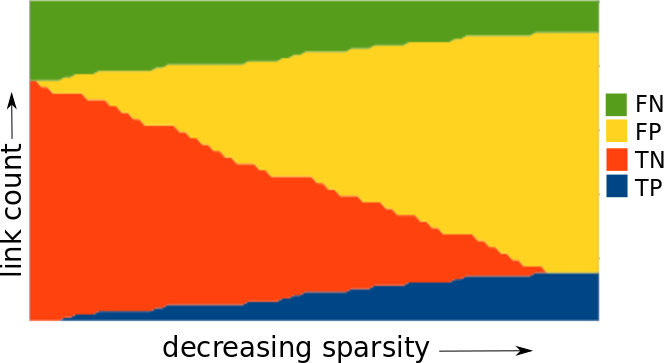
\includegraphics[width=1\linewidth]{4/confusionMatrix_sparsity.png}
\caption{\textbf{Generic confusion matrix in plot form across sparsity levels.} The sparsity decreases left to right. In this example, you see an initial empty network (leftmost) forced to sacrifice any true positive (TP) link in place of capturing all true negatives (TN). As links are added (moving right), some false negative (FNs) are exchanged for TPs or false positive (FPs), while other TNs are shifted to FPs as links are forced into the network as it becomes full. Every inference method starts and ends with these network makeups, the empty network a mix of FN and TN, while the full network cannot by definition contain TN. The intervening space is unique per inference method and its parameter setting. Thus finding the most accurate network is a method of balancing the ratio of these links whereby your any metric of accuracy estimation returns an optimal score.}
\label{fig:confusion}
\end{figure}

These individual link scores can be summarized and placed in relation to one another in various ratios. For the purpose of scoring each network individually we chose to report accuracy using Matthews correlation coefficient (MCC) (\cref{eq:MCC}) defined as follows,

\begin{equation}\label{eq:MCC}
MCC=\frac{TP*TN-FP*FN}{\sqrt{(TP+FP)(TP+FN)(TN+FP)(TN+FN)}}.
\end{equation}

This is a somewhat different approach from the inference summary statistics AUROC (\cref{eq:AUROC}) and AUPR (\cref{eq:AUPR}) which rate accuracy across all network sparsities as follow,
%  \begin{subequations}
\begin{equation}\label{eq:TPR}
TPR=\frac{TP}{(TP+FN)},\\ \end{equation}
\begin{equation}\label{eq:FPR}
FPR=\frac{FP}{(TF+TN)},\\ \end{equation}
\begin{equation}\label{eq:AUROC}
AUROC=\sum{TPR*FPR^T}
\end{equation}
% \end{subequations}

%  \begin{subequations}
\begin{equation}\label{eq:PPV} 
PPV=\frac{TP}{(TP+FP)},\end{equation}
\begin{equation}\label{eq:AUPR}
AUPR=\sum{TPR*PPV^T}
\end{equation}
%  \end{subequations}


When one does not have a true gold standard to measure accuracy against, we devised a \emph{cross validation} method and ultimately use the weighted residual sum of squares (wRSS) (\cref{eqn:wRSS}) in our error balancing procedure when estimating inference accuracy on the novel MYC dataset in \textbf{Paper III}.

\begin{equation}\label{eqn:wRSS}
  \textrm{wRSS}(\zeta) \triangleq \sum_k \frac{||-\bA^{-1}\hat{\bP}_k-\bY_k||^2_2}{cov(\by_k)}+\frac{||\hat{\bP}_k-\bP_k||^2_2}{cov(\bp_k)},
\end{equation}
%   \frac{||\hat{\bP}_k-(\bF_!k\bP^{-1}_{!k}\bP_k)||^2}{cov(\bp_k)}.

where $\hat{\bP}=(\bF_{!k}\bP^{-1}_{!k}\bP_k)$. Keeping with MCC, wRSS is made per network, and thus to evaluate across all sparsities like AUROC or AUPR the cumulative density can be calculated, summing the wRSS per network type. An explicit description of how this is calculated in a cross-validated way is described in the following Author's Note, explicitly walking through the BalanceFitError algorithm of \textbf{Paper III}.\\

\vspace*{5mm}
\fbox{\begin{minipage}{\linewidth}
\label{note}
\textbf{ Author's Note:}\\
The balancing algorithm in \textbf{Paper III} proceeds by stepwise up and down weighting the limit of the RSS of $\mP$, which constrains $\norm{\mF}$, whos addition to $\mE$ is minimized while solving the equation. Although the limit on $\mE$ is fixed, as the limit on $\mF$ fluctuates, so the smallest solution of $\mE+\mF$ which can solve the equation fluxes. So while $\mE$ starts small when $\mF$ is large (medium weighting), as the limit of $\mF$ becomes smaller (less weight towards RSS $\mP$ limit), $-(\mP-\mF)$ becomes more negative, which means to remain equal to $\mA(\mY-\mE)$, $\mE$ must become bigger, shifting weight from $\mF$ to $\mE$. The trick in inferring genes not present in the cross validation data comes in solving for them as the linear combination of cross validation genes, here  $\hat{\bP}$. In order to alleviate reproducibility bias which arises when the \emph{convex} solution is left otherwise \emph{underdetermined}, this estimated experimental error is balanced as a proxy for the distribution of noise to be expected on the inferred network. \emph{Gradient descent} is implemented using the CVX \emph{convex optimization} \citep{grant2008cvx} MATLAB \citep{MATLAB2017} package to this end. Networks returned are then fit to original data via CLS (\cref{eq:CLS}) to compare against null. 
% \caption{Author's Note}
\end{minipage}}\\


% \begin{figure}
% \centering
% 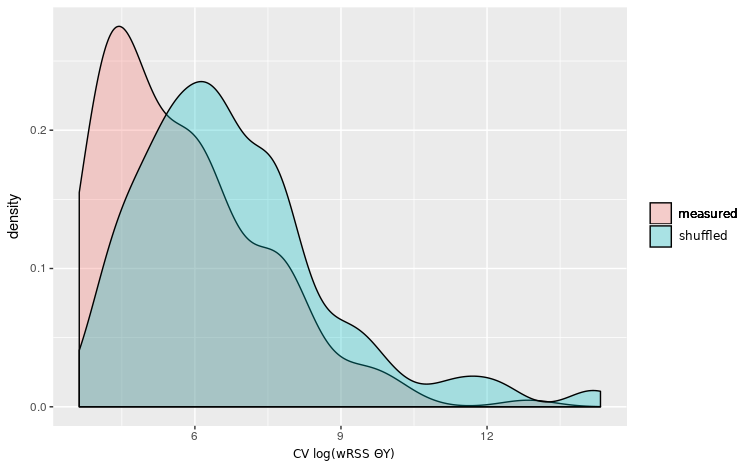
\includegraphics[width=1\linewidth]{4/allDensity_infVrand.png}
% \caption{{\textbf Cumulative Density of wRSS for true Y.} The overall sum of wRSS for all networks of types inferred (red) and random (blue), showing a lower overall error rate for measured networks across all sparsities.}
% \label{fig:CDF}
% \end{figure}




% Frobenius Norm
% Jacobian
% Determinant → schur decomposition
% Chi2inv→ chi2 has cross table structure
% -A-1

% \subsubsection{Ambiguous Benchmarks}
      
% \externaldocument{4/chapter4.tex}
\chapter{Present Investigations}

\section{GeneSPIDER - GRN inference benchmarking with controlled network and data properties (PAPER I)}
GeneSPIDER is a package developed for MATLAB to offer an outlook-proof environment for comparing inference algorithms. Some 15 modern inference methods are included and any number more can be easily added to this end. This benchmarking ability is made possible by a synthetic network and dataset creation pipeline with the ability to tune many properties therewithin. This informs the user when analyzing experimental dataset which methods and settings are appropriate for optimal inference. 
The controlled creation of dataset and networks of various sundry properties allows for an unbiased appraisal of any given method's accuracy in data-based network reconstruction (via \crefrange{eq:MCC}{eq:AUPR}, among others). Data properties owing to this performance can then be picked out when parameters are satisfactorily varied, and used to inform inference when gold standard networks are not available for accuracy measure, \ie inferring networks from biological dataset. The environment can also inform the scientist of experimental properties such as replicate number which will make downstream network inference more reliable and accurate.
A benchmark of methods across SNR, topology, size, and condition number showed many methods struggle to infer a network with accuracies better than random (50\% accuracy) when the SNR is significantly low, \ie low 0.01. This should lead scientists to strive for ever more higher fidelity transfers of genetic information to quantized datasets ultimately feeding into computer models, \ie through more experimental replicates. It also lead us to investigate ways of boosting inference accuracies by modeling the randomness many times to negate its effects, as well as weighing the costs of removing some genes shown to be especially noisey.

% \subsection{Outlook}

A major effort has already been made to incorporate more methods into the toolset. However, until these tools are freely available to the larger community of bioinformaticians, they will remain largely underutilized. A minor effort has been made to opensource this package to python, and a greater push is now needed if it ever hopes to gain adoption.


\section{A Generalized Framework for Controlling FDR in GRN Inference (PAPER II)}

NestBoot applies a bootstrapping protocol to any inference method to assess the stability estimated support values in order to mount a challenge to the many challenges uncovered in the GeneSPIDER benchmark, namely improving inference accuracies under poor SNR such as biological datasets. NestBoot inference is based on comparison of inferred networks from measured data to those inferred based on randomized data, which provides a sense of attaining such a network by chance. This allows for the control of FDR in a highly conservative formulation by comparing bootstrap support values to those of the same pipeline fed with shuffled data. This approach saw increases in regression methods: LASSO, LSCO and RNICO as well as tree consensus method Genie3 and the MI based CLR. across every SNR level, although increases were not uniform in their step.

% \subsection{Outlook}
The initial NestBoot protocol was implemented in the few methods benchmarked in the GeneSPIDER paper. However, they were restricted in many ways and quite heavy computationally. Furthermore, as the number of methods expanded, so too has the need for a more universal nested bootstrap adapter. A newer version now contains parameters to enter any method incorporated to GeneSPIDER, as well as a few methods which attain major speed boosts when operated over GPU utilizing native MATLAB CUDA functions. 

\section{Perturbation-based gene regulatory network inference to unravel oncogenic mechanisms (PAPER III)}

Our previous investigations of inference performance suggest optimal experimental design of many replicates mixed with partial knockdown. To this end, 40 genes known to have some involvement in cancer progression were perturbed with siRNA in triplicate. This allowed for network inference using three current methods. Accuracies were determined through a comparison not to true gold standard network, since none exist, but instead in a leave out manner to the original and validation datasets of the same gene compositions. This was accomplished by minimizing the error both of experiment read and inference, \ie E and F errors on Y and P, respectively. Since error can only be estimated from variances among Y matrix replicates, balancing of error was done to estimate inference errors, F.

Here, a common set of genes was perturbed and measured independently in human squamous carcinoma cell line. The training dataset contains genes perturbed and measured three times as experimental replicates, while the validation dataset contains the same genes perturbed in pairs without replicate. Taking into account various data properties, the training dataset was used to infer a network of the underlying mechanisms of control. This network was able to reproduce its training data in a leave out manner, and whatsmore, it is robust enough to reproduce a separate validation dataset to a degree of accuracy higher than expected by chance. In this way, many known links were recovered during the inference, as well as novel links proposed, two of which were verified experimentally. 

% \subsection{Outlook}
A major contribution of this paper is in the form of the knockdown dataset, performed some years ago on the technology of that time. Today, a incredibly powerful technology has been discovered and developed for targeted knockdowns far more precise than siRNA. CRISPRi offers the targeted knockdown of siRNA without the various off-target effects, and at a reduced cost. For the cost of personnel time to design primer sequence tags and carry out interference protocol as well as ordering primers the experiment can be done in multiplex, creating a new dataset of many more replicates for the same cost as the triplicate siRNA experiments of days past.


% \section{Large-scale Gene Regulatory Network Inference Reveals General and Specific Oncogenic Mechanisms (PAPER IV)}

% The L1000 offers a trove of richly characterized gene perturbation data, singly knocked down on a scale much larger than previously investigated here. Inferring a gene regulatory network (GRN) from this data grants insight into specific mechanisms directing cellular behavior in each of these disparate cell types. Networks are inferred from these 9 human cancer and 2 stem cell lines to explore the differences among human cancer GRNs. This is carried out in a reliable way using the NestBoot inference protocol for inferring individual cell line GRN by restricting the inclusion of false links. A comparison between these 2 healthy samples and cell line specific networks formed among these 9 cancer subtypes is made to find regulatory elements common among cancer types. Finally, an jacardian all-versus-all comparison is used to contrast specific regulators within each cell line to those in the healthy network. The results confirm many relational elements per specific oncogenic subtype, as well as novel regulations predicted within each cell line. However, up to this point we see a disparity in the degree distribution per inference method, namely that where LSCO presents mega-hubs, nodes with many outgoing regulatory links. This appears to reliably occur with N>100, where such gene lists would find unreliable relations inferred under such inference. This is an ongoing study and presents many mathematical questions. %Such findings made in the reliable fashion offered under NestBoot offer keys to identifying universal pathways involved in cancer progression and possibly even progenesis.

% % \subsection{Outlook} 

% Verifying such novel, inferred interactions would obviously be the first step in validating such reverse engineering. Further, utilizing the drug perturbation information for a screen of potential drug repositioning is a likely source of novel insight into the known and unknown treatments of compounds already in circulation amongst the world population. A primary outcome of interest would be in identifying drugs which inversely target the same patterns perturbed under certain cancers. Such would signals a dualism in the cause of the disease and its potential treatment, \ie the antagonistic relations targeted by each. Furthermore, finding drugs which actually have the same effect as disease would be an interesting discovery in so far as creating model organisms for outlook study. A simple dosage could present similar enough symptoms to offer manageable phenotypic models for developing treatment. 

% Tools comparing networks beyond n{\"a}ive link-link analysis are powerful and a perfect fit here. Specifically, ALPACA seems a great compliment and expansion of the present work, where networks inferred from different cell lines describing different tissue derived cancers are compared for module similarity. Further expansion could see MONSTER used to find transitions between time points recorded in the L1000 dataset, thought presently not containing inferred networks. Possibly state transitions between distinct cell line networks describing the same cancer could be estimated as well.


\section{A Subset Selection Method for Accurate Gene Regulatory Network Inference from Uninformative Datasets (PAPER IV)}

The L1000 \citep{subramanian2017next} offers a trove of richly characterized gene perturbation data, singly knocked down on a scale much larger than previously investigated here. Inferring a gene regulatory network (GRN) from this data grants insight into specific mechanisms directing cellular behavior in each of these disparate cell types. We used the L1000 data where roughly 978 genes were perturbed and subsequently expression levels quantified in 9 cancer cell lines. Key properties of the datasets, namely, signal-to-noise ratio (SNR) and condition number which we have shown to affect the performance of various inference methods were identified with the idea to maximize performance by optimizing each factor. 
In order to improve the poor SNR of the dataset we developed a gene reduction pipeline which eliminates the uninformative genes from the system using a selection criteria based on SNR until reaching an informative subset. We present a pipeline which identifies an informative subset in an uninformative dataset, improving the accuracy of the network inference.
This is quite opposing the quest to infer genome-scale GRN and possibly the best practices of data science regarding discarding data. However, until methods are created which can adequately handle noise on this scale (not an insurmountable challenge for \textbf{Paper II}), this is a first step in the direction of isolating probable submodules within a greater GRN yet to be uncovered.
% this file is called up by thesis.tex
% content in this file will be fed into the main document

%: ----------------------- introduction file header -----------------------
% \externaldocument{1/introduction.tex}
\graphicspath{{6/figures/}} % specifies where the figures are stored

% ----------------------------------------------------------------------
%: ----------------------- content ----------------------- 
% ----------------------------------------------------------------------

% \chapter{\label{ch6}Afterward} % top level followed by section, subsection

\chapter{\label{}Afterwards}

% \subsection{\label{}Name of subsection}

Boltzmann showed that entropy is what we really count when we delineate units of time. Furthermore, it has recently been proposed \citep{connes1994neumann} that this increase of entropy we envision for the universe is simply a bias toward the order which we have evolved to identify and thus find meaning in. Rovelli further postulates that the future may be no less ordered, and that there is no change in total entropy \citep{rovelli}. Order simply manifests in new ways, as in binning socks by color, only to have a colorblind man later bin them by length.

A construct of the human mind or not, the continuum we inhabit begs for understanding, to learn the behavior and boundaries of the perpetual change that is life. The GRN presented here are inferred using steady-state mechanics. Many factors are overlooked in the name of simplicity (see \cref{sec:regwhatwhen}, least of which is cell cycle synchronization, to measure separate experiments through similar periods of cell development and presumably under similar GRN regulation. This can be accomplished through starvation, \eg media deprivation forcing cells to recover from same stimuli together and thus bring their growth phases into sync. Such a uniforming starting point would allow time-series experimental quantification beyond simple assumptions of steady-state. This would enable modeling of relationship permanency, \ie if links are static, or more likely, if links are as transient as the condition the living systems finds itself inhabiting. This is one of the capabilities we have witnessed in the vastness of new high dimensional public datasets, \eg the LINCS project \citep{subramanian2017next}. Its high-throughput multiplexing has many time points taken within cell lines, which can feed into a model of network evolution, how links come into being, and thus a potential roadmap for which network conditions preclude any given network outcome.
%%drugL1000
The LINCS consortium also provides in its L1000 portal small molecule and drug induced perturbation experimental measures in keeping with the shRNA measures (see \cref{sec:ODE}) we use in \textbf{Paper IV}. It would be very interesting to develop a method for modeling drug perturbation on a network template, which could then be cross-correlated with inverse regulatory interactions in disease. Such pairing of disease and drug information in the context of networks could provide not only novel drug gene-targets, but also open the ability of less specific drugs targeting general network modules to achieve the same aim of changing the regulation of key disease pathways.

One straightforward method to achieve this using the similar models as those implemented here would be to code perturbation design onto small molecule, drug induced perturbation by way of the STITCH  \citep{kuhn2009stitch} or DrugBank \citep{wishart2006drugbank} databases. Creating such network models based purely on replicate, multiple perturbation experiments could uncover novel uses for drugs which have passed FDA phase I and II safety testing, thereby bypassing many years of safety testing not to mention chemical/structural development \citep{oprea2011drug}. These could then be very easily validated, at least in a rudimentary way through IC50 assay (50\% inhibitory concentration test) on the various standardized cell lines.
%%NN inf
Beyond perturbation-based inference methods, classic perception neural networks may hold key to further enhancing inference accuracy \citep{grimaldi2011regnann}, \citep{hache2007reconstruction}. Assembling a few layers to account for ingoing and outgoing links, strength as weights and up or down regulation would be easy when matched with a bank of sufficient training data. GeneSPIDER (\textbf{Paper I}) could be such a key, allowing for the creation of sufficient synthetic data for training with hold-out allowing for accuracy evaluation before feeding in real biological data. Furthermore, a bootstrap method drawing from experimental replicates would increase the training data amount as well as feed in a level of robustness where a network can describe many datasets due to varying levels of noise, combinations of experiments.

% \noindent\rule{12cm}{0.4pt}
\noindent\hrulefill

These past years I have been inspired to study many of the concepts present herein without directly identifying them as such. Specifically, I can recall that over the past year I spent compiling these chapters I been inspired by various forms of pop culture. These works reinforced what might be obvious, that genes (or anything else for that matter) do not and cannot exist in isolation. Moreover, despite the scientific method all but requiring it, any study done in isolation limits the aims and/or scope of the very study being done. Only as I saw this idea present itself in different domains again and again did I come to understand the repercussions. I was first so inspiration through what I have referenced formally from Carlo Rovelli's Order of Time\citep{rovelli}, which I followed reading Nick Pyenson's Spying on Whales\citep{pyenson},  and then Richard Powers' The Overstory\citep{powers}. These cultural works compliment very well what my studies suggest, a position to the much belabored quandry ``nature vs nurture'', which would seemingly posit that, like the idea that time is an artificial construct of the human mind or the age-old question ``what is the meaning of life'', there can be no separation of the two, nature and nurture, and these are simply bad questions. More specifically, the challenge we strive to collectively overcome is modeling complexity in our natural world, whether it be turbulent airflows or disease \emph{in vitro}. Thus changes to the system should be minimized to ensure the system maintains as many of its initial wild-type properties as possible, \eg culturing practices no matter how stringent the protocol, alters the system under study. Similarly, studying a tree isolated from its forest brethren does not characterize the wild-type individual just as investigating an orphaned and abandoned whale calve in captivity fails to capture its true nature. The encompassing system is composed of individuals which are themselves reflections of the constraints dictated by the environment. More to the point, there is no suitable nature without a nurture for it to grow and thrive within, the two are infact two sides of the same coin, as previously alluded to in the very beginning of \cref{sec:intro}.

We have understood that genes can maintain function over evolutionary time in similar species, \ie functional persistence, which allows transfer of function between newly characterized species within this similarity constraint; however, as equally well know, outside these similar species the gene, protein, \etc can and may very well develop entirely new functions. This demonstrates just how important the environment is to the function of any biomolecule, and thus how crucial it is we faithfully model the interactions within that environment. Such investigation, not excluding or excusing that presented here, often fall short of generalizing to the question initially posited, calling upon statistical tests to determine meaningful insight gained from the abstractions they become; nevertheless humanity's best approaches do over time consistently yield understanding, and as the tide of progress is never completely forward, we must endeavor to push on.

% The contributions I have made to the field are: 1) the creation of GeneSPIDER an environment for comparing inference methods; 2) NestBoot, a framework for enhancing many inference methods’ accuracy; 3) BalanceFitError (BFE), a method for measuring accuracy of inferred networks when gold standards are unavailable. GeneSPIDER has developed into the benchmarking environment for the consequent two projects. The NestBoot method initially found only a marginal ability to increase inference accuracies by comparing the network overlap across bootstraps. It was redesigned to implement a more strict thresholding manner by forming a null network distribution from the inference of networks based upon shuffled data, lending to the ability of the NestBoot framework to infer accurate networks by defining a way to enforce a naive but conservative FDR threshold. Similarly, BFE aims to overcome the limitation of scoring inference accuracy when no gold standard network is available by developing another null. Unlike our NestBoot null, here GRN links are shuffled after the initial inference to form a null expected-link distribution by which to compare any inferred network’s link composition, allowing us to score the ability of an inferred network to explain data relative to an expected error defined by this null distribution.

% Networks are all around us. In fact, you may count yourself part to any number without realizing. The modern incantation of social networks as omnipresent and unavoidable realities is just the latest example demonstrating the power relationships continue to carry as the basis for society, and viewed the right angle, for all life. One has only to propose a new perspective and relationships between constituent members will present themselves. Such members and their relationships can be summarized as networks, relational structures which allow for calculation, comparison and even prediction between and among members. When the interaction is obvious, forming a network requires little more that the will to compile. However, when the forces at work are a bit more esoteric, say in the realm of living physiology, witnessing the components is challenging enough, let alone characterizing their interplay. Yet this is precisely the matter discussed in this thesis, methods and tools devised and being devising to tease out relationships between the materials of life, for which here we mainly consider genes.

% All things must pass, and while I could never have imagined such a productive and exciting period of my life, it is with great excitment that I move on to the next adventure holding Stockholm close to my heart and her sensibilities forever in mind.


% In what I see as the culmination of my PhD studies, I have spearheaded a fourth study, which leverages experimental replicates within a high dimensionality public dataset. Utilizing a less pre-processed version of the data and normalizing in such a way that does not pool replicate experiments, we feed these replicates into our NestBoot FDR-enforcing inference framework. This creates cell type specific GRN, contrasting which allows for the search of conserved links and even modules. My greater ambition for this and any GRN project is to expand and infer using more input data types, and perhaps estimating regulatory dynamics using several time point rather than the steady state our model assumes. Identifying modules common among or specific to any cancer subtype GRN structure could expand the search space when identifying targetable biomarkers. A practical, testable application of biomarker identification in this manner would then be the integration of non-specific, small molecule perturbation data to enable the identification of novel drug-disease matches, \ie repositioning. While this is an ongoing investigation and not included here, it is my ultimate ambition to infer GRNs on whole genome level.

% I have been inspired by the robust relationships present in our natural world, in the way forest root systems propagate between individuals to form reactionary defenses against invasive species and how whale pods can communicate long term relationships among individual members...\\

% Future work hopes to involve the akaike and/or bayesian information criterion (AIC/BIC) to further bolster our results away from any bias we may introduce in our current estimations of inference performance, etc.


% ---------------------------------------------------------------------------
%: ----------------------- end of thesis sub-document ------------------------
% ---------------------------------------------------------------------------


% Include as many chapters as you need
     




% --------------------------------------------------------------
%:                  BACK MATTER: appendices, refs,..
% --------------------------------------------------------------

\backmatterSU

% the back matter: summary and references close the thesis

% Thesis summary -------------------------------------

% Should be in swedish if thesis are in another language, otherwize in english.
\selectlanguage{swedish}

%\summarytitle{Summering}

%\begin{summary}        %this creates the heading for the declaration page
\chapter{Sammanfattning}
Ur en ursprunglig, oenhetlig oordning, verkar ordning upprepade gånger ha uppstått i universum som en effekt av fysikens lagar. Där entropin hade föredragit att tomrummet förblev tomt, började kroppar smälta samman i allt större utsträckning, vilket ökade ordningen. När allt tyngre ämnen började fylla tomrummet, skapades en tillfällig stabilitet som motverkade entropins slutgiltiga mål genom att sprida ut materia här och där. Över tid ersattes ordning av större ordning, ända till den största triumfen över entropin skedde: livets uppkomst! (Eller det verkade så till en början: det har nyligen argumenterats för att liv istället ökar den samlade entropin fortare än frånvaron av liv skulle göra \citep{england2013statistical}) Sedan uppkomsten av replikation och självreplikerande biomolekyler har antalet hoptvinnade relationer ökat häpnadsväckande, och varje ny anpassning ger nya användningsområden för nya och gamla beståndsdelar, levande såväl som icke-levande (dvs konkurrens, symbios, parasitism etc). Dessa relationer existerar inom nästan varje nivå av liv, från djurplanktons avhängighet på tidvatten och månen till vårt samhälles beroende av uråldriga reserver av kolbaserad energi; återigen, ingenting i naturen existerar i ett vacuum.


Sådana typer av relationer kan kartläggas, katalogiseras och analyseras med hjälp av nätverk. Ett nätverk fångar upp flexibiliteten hos kraftfulla system in i en enda struktur; detta betyder dock inte att nätverk innebär förenkling; faktum är att många nätverk är så kompakta av förbindelser att de själva motsätter sig tolkning, just såsom de system som de beskriver \citep{dianati2016unwinding}. Varje system som innehåller två komponenter kan summeras som ett nätverk, med varje komponent sedd som en nod och deras relation till varandra som en länk. Olika vikter och konstnärliga utsmyckningar kan ges både till noder och länkar för att öka den kombinerade densiteten av information, men det är själva modellen av det totala systemet som ger mening till nätverket. Till exempel, när alla länkar är inräknade kan man ana den sociala påverkan av en nyhet, hur rikedomar sprider sig mellan släkter i utvecklingsländer, och av speciellt intresse här, hur gener fullgör instruktionerna som finns kodade i vår livskod. Vad händer när en specifik gen nedregleras – finns det då något annat sätt som gör att den kommer till uttryck, eller är systemet för alltid förändrat, dömt att anpassa sig eller till att helt enkelt ha mist sin funktion? Och när kombinationen av sådana reaktionsvägar förändras, hur har systemets överlevnadsinstinkter förberett det? Biologiska system av alla storlekar har visat sig vara mycket stabila, vilket man intuitivt kan gissa från vidden på mänsklig föda eller bredden av människor, djur och olika språk på denna planet. Genregulatoriska nätverk (GRN) är inget undantag. Faktum är att mäta en gens relation till en annan, dvs kartlägga dess lokala nätverk, är extremt svårt just på grund av detta, att relationerna passerar många mellanspelare och ofta är sammansatta genom unika loopstrukturer som förstärker deras relation. 


Verktyget GeneSpider i \textbf{Paper I} försöker erbjuda en viss tydlighet för att lösa denna uppgift, genom att ge lika villkor för att testa många olika metoder av nätverksinterferens, i hopp om maximal pålitlighet. Verktyget tillåter  generation av  syntetisk data vilken speglar många egenskaper som finns i verklig experimentellt framtagen biologisk data. Denna data tillåter full kontroll i skapandet av nätverk , något som ofta saknas i faktiska experiment och ger en uppskattning av noggrannheten. Nutida metoder av nätverksinterferens varierar på många olika sätt, ingen mindre trivial än dess anslag av variation i mätningar. Vårt ramverk för FDR-kontroll i nätverksinferens i \textbf{Paper II} mäter denna variation inom frekvenser tillräckliga noga för att ge den underliggande inferensmodellen  en god uppskattning av den inneboende variabiliteten för systemet. Vilket ger tillbaka ett pålitligt nätverk baserat på strikta kriterier för att acceptera falska nätverkslänkar. Den störnings-baserade interferens metoden presenterad i \textbf{Paper III}  studien är kulmen av denna och annan forskning, alla som guidats av experimentell design, genom inkluderandet av många replikat av individuellt brus. Dessa data behandlades i verktyget ”FDR restricing framework” för att ge ett pålitligt nätverk som mäts mot en strikt korsvalideringsmetod. På samma sätt kan användandet av dataegenskaper för att begränsa inferens till endast den som kan uttydas med rimlig noggrannhet möjligen leda till en större acceptans inom fältet (\textbf{Paper IV}) och därmed mindre motstånd när man går vidare till den kliniska domänen. Att ta bort mycket experimentell data kommer onekligen skapa frustration men det kan också leda till en revolution för större experimentellt djup inom biologisk karakterisering. \\


\noindent{översatt av Malin Lundahl och Sofie Wendel, med ytterligare redigering av Thomas Hillerton.}



%\end{summary}

\selectlanguage{english}

% ----------------------------------------------------------------------

% Thesis Acknowledgements ------------------------------------------------


%\begin{acknowledgementslong} %uncommenting this line, gives a different acknowledgements heading
%\begin{acknowledgements}      %this creates the heading for the acknowlegments
\chapter{Acknowledgements}

I would not have been able to complete this work without my immediate family. My brother Evan visited the first and third summer of my study, the second of which trip lasted nearly 10 weeks as he studied during the day and joined in climbing and exploring the city by night. His strength and unwavering love and encouragement made the summers that much more exciting, as have video chat these past years made the dark winter months that much more bearable. My mother Cynthia and father Thomas provided much the same. From their encouragement I strove to continue studying year after year rather than jump to industry and the constraints of \emph{real adult life}. Even as they pushed to be a financially responsible adult and consider more conventional jobs in industry, I clung to academia in a move towards quite the opposite. More than that, my mother taught me early on teaching that good arguement is key to logical discourse. That it's not enough to make sense to yourself but that communication is check against insanity, not to mention spreading good ideas. For his part, my father taught me to look up into the canopy of a tree as you walked by, to marvel at the everyday and question its being. Second only to this family is my neighborhood family, the Osbornes: Big and little Larry, Kathy and Meredith (and now Adam and Clark), have been friends, siblings, parents and second or extended family.
%%Core Sonnhammer Group
Toward the matter of completing the work, I must thank Erik Sonnhammer above all, for giving me the opportunity and time to learn and grow as a scientist, ascending quite the learning curve toward our shared goal of contributing to the field. Equally, I must thank Sweden for investing in a foreign born son who has been made to feel very much welcome and part to the society and culture. I took the position never having breached the confines of the continental U.S., and only after four years do I realize I could not have found a more welcoming new home. It is amazing such financing and support for foreign scientists exists in a world so wrought with divisiveness that the mirror process in my home nation is far from common. It is my intention and indeed my deepest hope to one day return and repay this wonderfully open society for its investment. Also to my co-supervisor Torbj{\"o}rn Nordling for hours of one-on-one tutoring, both in person and via skype. Visiting his young lab filled with bright-eyed undergraduate and masters students was one of the highlights of both my research and personal life, solving a crucial piece of the validation in \textbf{Paper III} as well as meeting many new hiking, travel, street workout, late-night eating and generally adventurous friends in the process. Similarly, this research is heavily indebted to that of Andreas Tj{\"a}rnberg, whos guidance during the early days of my GRN life proved invaluable to my understanding and ultimately to these contributions. A latecomer to the group, Deniz Seçilmiş seemed bound to be to me what I was to Andreas, yet, she has surpassed this initial estimation in almost every way, teaching me so much along her way toward becoming a self sufficient methodologist. I anticipate future collaboration with this core team as I very much hope to maintain regular communication as we have these past years, delving deeper into the possibilities contained within the GRN field and beyond. Lest I forget SU faculty, including Gunnar von Heinje, Erik Lindahl, Pia {\"A}delroth and Stefan Nordlund, as well as IT support Stefan Fleischmann and Erik Sj{\"o}lund, and secretaries Alexander Tuuling, Maria Sallander and Elisabeth Johansson.
%%Other Sonnhammer Group
Friendships from within the Sonnhammer group at large has been a major source of encouragement along this road, including friendships I hope to last my lifetime. Namely that of Christoph Ogris and his beautiful wife Lisi, who took me in much like a lost puppy during my first harsh Swedish winter, sharing with me their passion of rock climbing, hiking and general enthusiasm for all things natural. Their relationship is another example to my eyes of determination in ones life, being decisive in intent then following up to make sure it works out. I would not be who I am today without their friendship. Furthermore, seeing Christoph in his natural habitat (the Austrian Alps of Schladming) gives me a better appreciation for the simple pleasure to be had over dinner, wine, fire and snow with friends in nature. In those early puppy days I looked up to Christoph like an older brother, and now that we have both summited mount doctorate I hope that our shared experience proves a bond all the stronger. They even introduced to now mutual friends Roman and Sandra, Swiss Chris and Maja. Similarly like being amongst family, the experience being welcome into the homes of both Deniz and Miguel during is something I will treasure. I gained such an appreciation for these amazing individuals seeing them in their respective \emph{natural elements} after having known them in the abstraction that is the (computational) lab environment. Similarly yet of a unrelated variety, Mateusz Kaduk and his bride to be Kate have offered wonderful friendship upon lab events and group outings in the city, most memorably visiting the Skansen for each beautiful pagan spring ritual derived from witch burning of olde. As a house-mate and long time Stockholm resident, Stephanie provided much startup help for my moving process as well as a wonderfully unique perspective on all things German and Soviet, both past and present, not to mention the swimming classes she gave for Lisi, I and universtiy students. Lest I forget a major inspiration not just for science but for living life, Dimitri Guala and his relationship with his beautiful wife Izabela have shown what professional careers outside academia can look like and the lifestyle they afford, not just monetarily but in values of health and family. 
%%SciLifeLab
To my first lab friends, Annemarie Perez Boerema and Miroslav Huliciak, both of whom opened their homes to me for visits during various holidays. To Daniel Jans, David Jess for the many lunch time runs, and to the many other lab friends who would come to occupy the halls of our beloved Gamma 3, I thank you for your endless conversations, pondering each member's home country's latest election results, sharing fikas, cakes and beers at the pub night: Marta Carroni, Juni Andrell, Alex Muhleip, Narges Mortezaei, Victor Tobiasson, Jose Miguel de la Rosa Trevin, Giovanna Coceano, Francesca Pennacchietti, Jonatan Alvedlid, Andreas Boden, Steven Edwards, Liang Zhang, Evgeny Akkuratov, and a few of the floor's other P.I.'s Ilaria Testa and Alexey Amunts, the later who's application expertise helped me attain my first postdoc position. Other SciLifeLab \& DBB friends Mirco Michel, John Lamb, Marco Salvatore. 

Lest I forget my first contact in Sweden outside the lab, the woman who picked me up at the airport after my first international flight, whos brother drove me back into the city after I purchased a bike in disrepair via the pendeltag, who overlooked the security deposit when I was broke after arriving in Sweden a month before my salaried contract started; Ulrika Larsson was like my Swedish mother those first two years, and I cant imagine the hardship she saved me from during that time. Futhermore, to the Swedish people, firstly for enabling such a healthy period of learning, especially to a foreigner, through more than adequate funding; not to mention for making learning easy by practicing such good English that it is my great shame to have learned more Turkish over a ten day trip in 2018 that I have Swedish in 4.5 years.
%%Klatter
I thank the many climbing friends I have made inside the various klattercentrets as well as outside in the innumerable afterwork and weekend session throughout Stockholm and southern Sweden, many of whom I also shared scientific discussion as fellow students. Namely, Jacupo Fontana (another larger than life big brother type in my eyes) and his GF Franchesca, Giacamo Sitzia, Kaveh Rezania, Leo Sparring, and the dozen or so others I may have forgotten.
%%OSU
To my past PI's and advisors: John Letterio, Melany Fisk, especially Ohio State advisor Kun Huang and PI James Chen, professors Philip Payne and Albert Lai, and program secretary James Gentry who taught me the importance of paperwork efficiency. To my best classmate from this time, Marcelo Lopetegui Lazo and his wife Barbara, for their friendship, Chilean sentiment and fun times, skiing and partying. To my Ohio State friends Alan, Amy, Caleb, Carrie, Kyle, and Steve, for the endless nights discussing politics over mead, dancing out at concerts and generally cavorting through central Ohio. Many have visited me in Stockholm and abroad, always bringing an element of home along with them. To my best roommate, Jatin Gupta, who was an ideal role model of simplicity and loving life during his studies, not to mention the best chef in the area! To my OSU hockey brothers, especially Dane, Manuel, Eric and my closest bud Big John. He has introduced me to many of the luxuries of independent adulthood, least meeting new friends David and Christian while biking our way around Berlin. And to my college roommate Jeremy Verner, for reminding me that work ethic can being liberating rather than constraining. To my high school classmates and later friends in life, Corey McNeilley, Baz and Jack Masin, for teach me to surf and sail, for challenging me in political and philosophical thought, as well as in friendship when friends evolve. To my college hockey and rowing friends, as well as my high school rowing and rugby friends, for never letting me forget that pain does not have to be ones enemy.
%%BUD, DEB
To the memory of my grandfather Bud, whom this writing is dedicated to, who been a major force in my life without the two of us ever having met. A force of inspiration is key to my development, and the only equal in my life would be that of his second daughter's best friend, my aunt Debra, who has been my scientific role model since my first science fair entry (on geotropism, taking home second prize with the help of my father). My mother has long told me tales of her doctoral studies, which I carry with me and share retell to friends under stress, that tackling just ``one mouse a day'' day in and day out can yield grand accomplishments. And to her husband Fred who Fred who scaring me into realizing foreign institutions compete for same journal publications. To my grandmothers Helen and Irene, whos refrigerators and candy bowls were never empty despite having 15+ respective other grandchildren regularly ransack their homes, and to my grandfather Bob, who showed me such joy and friendship early on as his "buddyboy".

For all these and more wonderful relationships I am forever grateful; each means more than I could have imagined when I set out on this journey four and 26 something years ago, and I only hope for their continued prosperity.

And last but not least, an extra special thanks to Miguel Castresana Aguirre Bengoechea Lasa Eguia Arocena Garbizu Imaz Elola Balerdi Arrayago Garmendia Txapartegui Retegui  ... for being Basque.
%\end{acknowledgements}
%\end{acknowledgmentslong}

% ------------------------------------------------------------------------


  % Use this to include an acknowledgement in the backmatter

%: ----------------------- bibliography ------------------------

% The section below defines how references are listed and formatted.


%\begin{multicols}{2} % \begin{multicols}{ # columns}[ header text][ space] %uncomment to have 2 columns
\begin{scriptsize} % tiny(5) < scriptsize(7) < footnotesize(8) < small (9)

\bibliographystyle{Latex/Classes/PhDbiblio-url2} %Default style file. Change according to you preferences.


\renewcommand{\bibname}{References} % changes the header from Bibliography to References

\bibliography{9_backmatter/references} % adjust this to fit your BibTex file

\end{scriptsize}
%\end{multicols}


% Various bibliography styles exit. Replace above style as desired.

% in-text refs: (1) (1; 2)
% ref list: alphabetical; author(s) in small caps; initials last name; page(s)
%\bibliographystyle{Latex/Classes/PhDbiblio-case} % title forced lower case
%\bibliographystyle{Latex/Classes/PhDbiblio-bold} % title as in bibtex but bold
%\bibliographystyle{Latex/Classes/PhDbiblio-url} % bold + www link if provided
%\bibliographystyle{Latex/Classes/jmb} % calls style file jmb.bst
% in-text refs: author (year) without brackets
% ref list: alphabetical; author(s) in normal font; last name, initials; page(s)

%\bibliographystyle{plainnat} % calls style file plainnat.bst
% in-text refs: author (year) without brackets
% (this works with package natbib)


% --------------------------------------------------------------



\end{document}
